\documentclass[12pt]{article}


\usepackage[toc,page]{appendix}
\usepackage[nottoc,numbib]{tocbibind}
\usepackage{bbm}
\usepackage{stmaryrd}
\usepackage{xifthen}
\usepackage{wrapfig}
\usepackage{adjustbox}
\usepackage{array}
\usepackage[hidelinks]{hyperref}
\usepackage{amsmath}
\usepackage{amssymb}
\usepackage{amsfonts}
\usepackage{dsfont}
\usepackage{url}
\usepackage[a4paper,left=1in,top=1in,right=1in,bottom=1in,nohead]{geometry}
\usepackage[round]{natbib}
\usepackage{multirow}
\usepackage{algpseudocode}
\usepackage{algorithm}
\usepackage{subcaption}
\usepackage{pstricks}

\usepackage{booktabs}
\usepackage{colortbl}


%\let\emph\relax % there's no \RedeclareTextFontCommand
\DeclareTextFontCommand{\textbfit}{\bfseries\em}

\title{\textbf{What to Write and How to Write It}\\
       \textit{\large Modeling Content Selection and Generation for Text Summarization}\\
       ~\\
       ~\\\large\textbf{Thesis Proposal}}
\author{~\\
        \textbf{Chris Kedzie}\\
        Department of Computer Science\\
        Columbia University\\
        \url{kedzie@cs.columbia.edu}}

\date{December $10^{\textrm{th}}$, 2018}

%\usepackage{unicode-math}
%\setmathfont{XITS Math}
%\setmainfont{TeX Gyre Pagella}

% Any of the following work, and probably many more
%\setmathfont{TeX Gyre Pagella Math}
%\setmathfont{TeX Gyre Termes Math}
%\setmathfont{STIX}
%\setmathfont{Asana Math}


\begin{document}

\pagenumbering{gobble}
\maketitle

\pagebreak

\renewcommand{\thepage}{\roman{page}}
\setcounter{page}{1}

\begin{abstract}
  Automatic text summarization is one of the longest-standing 
application areas in the 
field of natural language processing (NLP), with a history as deep 
as some of the more foundational tasks, e.g. syntactic parsing 
\citep{yngve1955syntax} or 
part-of-speech tagging \citep{harris1962string}. 
While there are many variants, 
the general summarization task is 
to reduce a large input text into its most essential pieces of information,
and in doing so reduce the amount of reading a human has to do. 
In this thesis we focus on advances to two summarization subtasks:
\textit{(i)} identifying the most import content for inclusion in the summary, 
and \textit{(ii)}
rendering that content in such a way as to not misrepresent the original 
input. We refer to the former as \textbfit{salience estimation} and the latter
as \textbfit{faithful generation}. 

With respect to problem \textit{(i)}
we propose two novel methods for working in low context, streaming
news scenarios using feature-based regression, clustering, and 
learning-to-search. Additionally, we develop several hierarchical models
of sentence salience using deep neural networks. We perform
analyses of different neural architecture choices in the context of 
single document summarization across multiple genres along with ablation
studies to understand what signals in the data are most important for
model training. Based on these experiments, we find impediments to learning 
useful lexical features at the sentence level, 
and propose a novel word importance model
with frequency and surprisal based feature embeddings to overcome these 
limitations. We also propose a method of domain adaptation of this word 
importance model 
from single-document summarization to multi-document summarization.

Finally, we introduce a novel framework for
generating text that is faithful, i.e. respects prior knowledge or input data, 
in an effort to provide stronger guarantees 
about summary reliability and prevent the hallucination of facts. 
In particular, we model generation as a two player
game between a \textit{generator}, 
a conditional language model that produces a 
text utterance given an input (either text or table data), and 
a \textit{recognizer}, a classifier that tries to accurately predict the 
original input data from the generator's utterances. 
We explore this framework in both data-to-text and text-to-text settings.
In the data-to-text setting, the recognizer tries to predict the values of 
fields from the conditioning table data, e.g. 
predicting someone's occupation from a brief
biographical description produced by the generator.
In the text-to-text setting, the recognizer answers cloze style questions
\citep{taylor1953cloze}
about the input text, given an abstractive summary produced by the generator.
The generator uses the recognizer as a learning signal to perform beam 
search optimization \citep{wiseman2016sequence}; the goal here is to learn a generator that is capable of
producing syntactically diverse utterances that respect the conditioning
input data. We additionally discuss how this framework can be used as an 
alternative method of controllable text generation, with the added benefit
that we learn a recognizer model that can give confidence scores about
the faithfulness of a given utterance.




\end{abstract}

\pagebreak

\tableofcontents
\newpage

%%% Latex Table Column Types %%%

\newcolumntype{g}{>{\columncolor{black!5}}c}
\newcolumntype{f}{>{\columncolor{black!5}}r}
\newcolumntype{L}[1]{>{\raggedright\let\newline\\\arraybackslash\hspace{0pt}}m{#1}}
\newcolumntype{R}[2]{%
    >{\adjustbox{angle=#1,lap=\width-(#2)}\bgroup}%
    l%
    <{\egroup}%
}
\newcommand*\rot[2]{\multicolumn{1}{R{#1}{#2}}}

%%% General Math Notation %%%

\newcommand{\fdef}[3]{#1 : #2 \rightarrow #3}
\newcommand{\R}{\mathbb{R}}
\newcommand{\Rnonneg}{\mathbb{R}^{\ge 0}}
\newcommand{\N}{\mathbb{N}}
\newcommand{\Npos}{\N^{+}}
\newcommand{\Rn}[1]{\R^{#1}}
\newcommand{\Ind}[1]{\mathbbm{1}\{ #1 \}}
\newcommand{\Idx}[1]{\llbracket #1 \rrbracket}
\newcommand{\Sze}[1]{| #1 |}
\newcommand{\E}{\mathbb{E}}
\newcommand{\entropy}{H} 
\newcommand{\dataset}{\mathcal{D}}
\newcommand{\objective}{\mathcal{L}}
\newcommand{\discSet}{\mathcal{X}}

%%% General Lang Processing %%%

\newcommand{\tfidf}{TF-IDF}
\newcommand{\idf}{IDF}
\newcommand{\meteor}{\textsc{Meteor}}
\newcommand{\rouge}{\textsc{Rouge}}
\newcommand{\rougeN}[1]{\textsc{Rouge-{#1}}}


%%% Feature Based Salience Models Macros $$$

\newcommand{\query}{q}
\newcommand{\Queries}{\mathcal{Q}}
\newcommand{\strsent}{s}
\newcommand{\sentvec}{\mathbf{s}}
\newcommand{\strsents}{\mathcal{S}}
\newcommand{\feats}{\phi}
\newcommand{\nugget}{n}
\newcommand{\Nuggets}{\mathcal{N}}
\newcommand{\nuggets}{\mathcal{N}}
\newcommand{\predNuggets}{\hat{\Nuggets}}
\newcommand{\extract}{a}
\newcommand{\salience}{y}
\newcommand{\predSalience}{\hat{y}}
\newcommand{\saliences}{\mathbf{\salience}}
\newcommand{\predSaliences}{\mathbf{\hat{\salience}}}
\newcommand{\salThresh}{\lambda_1}
\newcommand{\simThresh}{\lambda_2}

\newcommand{\gp}{\mathcal{GP}}


\newcommand{\Salience}{Y}
%\newcommand{\similarity}{k}
\newcommand{\Similarity}{\mathbf{K}}
\newcommand{\updates}{\mathcal{U}}
\newcommand{\update}{u}
\newcommand{\exemplars}{\mathcal{E}}
\newcommand{\similarity}[2]{\textsc{Similarity}(#1, #2)}
\newcommand{\sapcluster}[2]{\textsc{AffinityPropagation}(#1, #2)}


\newcommand{\comprehensiveness}{\textsc{Comprehensiveness}}
\newcommand{\expectedGain}{\E\left[\textsc{Gain}\right]}
\newcommand{\comp}{\textsc{Comp.}}
\newcommand{\fmeasure}{F1}

\newcommand{\sap}{\textsc{Sap}}
\newcommand{\ap}{\textsc{Ap}}
\newcommand{\ranksal}{\textsc{Rs}}
\newcommand{\hac}{\textsc{Hac}}

\newcommand{\modelLS}{\textsc{L2s}}
\newcommand{\modelLSCos}{\textsc{L2sCos}}
\newcommand{\modelCos}{\textsc{Cos}}

%\newcommand{\poi}{T}


%%% Faithful Generation Macros %%%
    \newcommand{\evidence}{x}
    \newcommand{\evidenceSpace}{\mathcal{X}}
    \newcommand{\evidenceSpaces}[1]{\evidenceSpace_1
    \times \cdots \times \evidenceSpace_{#1}}
    \newcommand{\utterance}{y}
    \newcommand{\gen}{p}
    \newcommand{\genParams}{\theta}
    \newcommand{\rec}{q}
    \newcommand{\recParams}{\phi}
    \newcommand{\vocab}{\mathcal{V}}
    \newcommand{\faithful}{\textsc{Faithful}}


\newcommand{\beamDistr}{\beta}


%%% Learning To Summarize
\newcommand{\policy}{\pi}
\newcommand{\policySpace}{\prod}
\newcommand{\lsAction}{a}
\newcommand{\lsActionSpace}{\mathcal{A}}
\newcommand{\oraclePolicy}{\policy^{*}}
\newcommand{\modelPolicy}{\hat{\policy}}
\newcommand{\rollOutPolicy}{\policy^{out}}
\newcommand{\lsState}{s}
\newcommand{\lsStateSpace}{\mathcal{S}}
\newcommand{\lsStep}{t}
\newcommand{\lsTrans}{T}
\newcommand{\lsSaliences}{\mathbf{y}}
\newcommand{\lsSaliencesRollOut}{\mathbf{y}}
\newcommand{\lsSaliencesRef}{\mathbf{y}^*}
\newcommand{\lsStrucLoss}{\ell}
\newcommand{\lsCost}{c}
\newcommand{\lsChoiceParam}{\beta}
\newcommand{\policyParams}{\mathbf{W}}
\newcommand{\lsFeats}{\phi}

%%% Deep Learning Models of Content Salience %%%

\newcommand{\sent}{s}
\newcommand{\Sents}{\mathcal{S}}
\newcommand{\doc}{d}
\newcommand{\lbl}{y}
\newcommand{\Labels}{\mathbf{y}}
\newcommand{\word}{w}
\newcommand{\extracts}{\mathcal{E}}
\newcommand{\budget}{c}
\newcommand{\encoder}{\textsc{Encoder}}
\newcommand{\extractor}{\textsc{Extractor}}
\newcommand{\embproj}{W}
\newcommand{\emb}{\omega}
\newcommand{\embsize}{n}
\newcommand{\sembsize}{m}
\newcommand{\semb}{\mathbf{h}}
\newcommand{\rsemb}{\overrightarrow{\semb}}
\newcommand{\lsemb}{\overleftarrow{\semb}}
\newcommand{\gru}{\textsc{Gru}}
\newcommand{\rgru}{\overrightarrow{\gru}}
\newcommand{\lgru}{\overleftarrow{\gru}}
\newcommand{\cfeat}[2]{\mathbf{f}_{#1}^{( #2 )}}
\newcommand{\relu}{\textsc{ReLU}}
\newcommand{\winsize}{k}
\newcommand{\winsizes}{K}
\newcommand{\fmapsize}{F}
\newcommand{\cfidx}{l}
\newcommand{\cact}{a^{(\cfidx,\winsize)}}
\newcommand{\cnnbias}{\mathbf{u}^{(\winsize)}}
\newcommand{\cnnweight}{\mathbf{U}^{(\winsize)}}
\newcommand{\cnnBiasSpace}{\mathbb{R}^{\fmapsize_\winsize}}
\newcommand{\cnnWeightSpace}{\mathbb{R}^{\winsize \times \fmapsize_\winsize \times \embsize}}

\newcommand{\extHid}{\mathbf{z}}
\newcommand{\rExtHid}{\overrightarrow{\extHid}}
\newcommand{\lExtHid}{\overleftarrow{\extHid}}
\newcommand{\demb}{\mathbf{d}}
\newcommand{\smemb}{\mathbf{s}}
\newcommand{\posemb}{\mathbf{f}}
\newcommand{\qrtemb}{\mathbf{c}}

\newcommand{\enextHid}{\mathbf{e}}
\newcommand{\deextHid}{\mathbf{d}}


%%sent enc
\newcommand{\enAvg}{\textsc{Avg}}
\newcommand{\enRnn}{\textsc{Rnn}}
\newcommand{\enCnn}{\textsc{Cnn}}

%%% Wimpy Models %%%
\newcommand{\elmo}{\textsc{Elmo}}
\newcommand{\glove}{\textsc{Glove}}

\newcommand{\bowvec}{\omega}


List of General Definitions \\


\begin{tabular}{l l}
    $\R$ & The set of real numbers.\\
    $\N$ & The set of integers.\\
    $\Npos$ & The set of positive integers.\\
    $\discSet$ & A generic discrete space. \\ 
    $\Sze{x}$ & Cardinality of a discrete set or sequence $x$. \\
    $\Ind{\cdot}$ & Iverson bracket, i.e. evaluates to 1 if proposition in brackets evaluates to \textsc{True}.\\
    $\Idx{n}$ & The index set $\{1, 2, \ldots, n\}$ for any $n \in \Npos$.\\
    $\E[\cdot]$ & The expected value. \\
    & When ambiguous we will use a subscript
                   $\E_p[\cdot]$ to specify the distribution $p$. \\
    $\entropy$ & The Shannon entropy, 
                    $-\sum_{x \in \mathcal{X}} p(x) \log p(x)$.
                  We will use the subscript $\entropy_{p(\cdot)}$
                 to specify the distribution if it is ambiguous.\\
    $\dataset$ & A dataset.\\
    $\objective$ & An objective function.\\
\end{tabular}

~\\

\pagebreak

List of Chapter 3 Definitions\\

\begin{tabular}[t]{p{1.1cm} p{13cm}}
    $\query$ & An event query string, e.g. ``Hurricane Sandy''.\\~\\
    $\strsents(\query)$ & A sentence stream, i.e. a time-ordered sequence of 
                 sentences for a particular query $\query$.
                 Typically we will omit the the query as it will be clear
                 from the context which stream we are refferring to.\\~\\
    $\strsent$ & A sentence from the sentence stream $\strsents$.\\ ~\\
    $\feats$ & A function $\fdef{\feats}{\strsents}{\Rn{d}}$ mapping 
                sentences to a $d$-dimensional feature vector.  \\~\\
    $\Nuggets(\query)$ & The set of nuggets associated with query $\query$.
                 Typically we will omit the the query as it will be clear
                 from the context which nuggets we are refferring to.\\~\\
    $\nugget$ & An event nugget text. \\~\\
    $\updates$ & A distinguished set of sentences 
                 $\{\strsent_i\}\subseteq \strsents$ that were emitted
                 by a stream summarization algorithm, i.e. the extract 
                 summary for a stream $\strsents(\query)$.\\~\\
    $\predNuggets$ & The set of nuggets contained by the predicted 
                    extract summary $\updates$,
                     i.e. $\big\{\nugget \in \Nuggets\ |\  
                        (\exists \strsent \in \updates)
                        [ \nugget \in \strsent] \big\}$.\\~\\
   $\salience$ & The salience of a sentence $\strsent$. Salience
                 scores are real valued.\\~\\
   $\saliences$ & A vector of $k$ salience values, i.e. 
$\saliences = (\salience_1, \ldots, \salience_k) \in \Rn{k}$.\\~\\
   $\predSalience$ & The predicted salience of a sentence $\strsent$. Salience
                 scores are real valued.\\~\\
   $\predSaliences$ & A vector of $k$ predicted salience values, i.e. 
$\predSaliences = (\predSalience_1, \ldots, \predSalience_k) \in \Rn{k}$.\\~\\
$\exemplars$ & The set of exemplars selected by the Affinity Propagation
                algorithm. \\~\\


\end{tabular}




\newpage

\renewcommand{\thepage}{\arabic{page}}
\setcounter{page}{1}

% Change to false to compile full document.
\def\highlevel{true}

\section{Introduction}

Everyday we ask friends and colleagues to do it, to tell us about books, 
newspaper articles, and other complex texts, and, without more than a 
moment's reflection, they are able to compress their experience
into succint natural language statements that describe the
subject of our request.
The ease with which we summarize belies the difficulty of
writing programs that do so, and so it would appear that 
the robust
ability to create summaries is, as of 2018, a uniquely human capability.
This partially explains summarization's allure to the artificial intelligence (AI)
research community, which has in one way or another, attempted to aggregate
and naturally compress text data since at least the 1950's 
\citep{luhn1958automatic}.
This makes automatic text summarization one of the longest-standing 
application areas in the 
field of natural language processing (NLP), with a history as deep 
as some of the more foundational tasks, e.g. syntactic parsing 
\citep{yngve1955syntax} or 
part-of-speech tagging \citep{harris1962string}. 

While there are many variants, 
the general summarization task is 
to reduce a large input text into its most essential pieces of information,
and in doing so reduce the amount of reading a human has to do. 
In this thesis we focus on advances to two summarization subtasks:
\textit{(i)} identifying the most import content for inclusion in the summary, 
and \textit{(ii)}
rendering that content in such a way as to not misrepresent the original 
input. We refer to the former as \textbfit{salience estimation} and the latter
as \textbfit{faithful generation}. 

The completed and proposed methods of salience estimation cover a range of
techniques including regression, clustering, learning-to-search,
and deep neural networks. 
We experimentally verify the utility of our approaches
across a variety of summarization tasks including stream summarization,
single-document summarization, and multi-document summarization.
The general research goal here is to develop flexible models for 
identifying
important words, phrases, and sentences that are likely to serve as 
representitive members of the larger text in which they are found.

In \textbfit{extractive summarization}, 
where the summary is constructed by copying and pasting phrases or sentences 
from the input text, salience estimation can be used directly to create
a summary. For example, a simple method of sentence extractive summarization
would be to order the input sentences by decreasing salience and select the
top few sentences for the summary. In most cases, salience is not the only
consideration for summary inclusion; redundancy, discourse coherence, fluency,
and many other metrics of text quality can and have been used as content
selection criteria. These measures are largely independent of salience 
(with the noteable exception of redundancy) and so we do not explore them in 
detail here. The details of our completed and proposed work on 
salience estimation can be found
in sections \ref{sec:feature_salience} and \ref{sec:deep_learning_salience}.

In \autoref{sec:feature_salience} we develop two feature-based models of 
sentence
salience and evaluate them in a relatively novel \textbfit{stream 
summarization} crisis-monitoring scenario
\citep{starbird2013working,aslam2015trec,aslam2016trec}. In this task, a user is interested
in tracking information about a disaster event (e.g. a hurricane). The
user provides a text based query describing the event 
(e.g. ``Hurricane Sandy'') to the summarization model. 
The model must then 
monitor a stream of news articles, extracting important sentences in the 
document stream and present them to the user. The information must be 
highly salient to the query event, as well as novel and timely to the user 
-- we do not want to bombard the user with irrelevant or repeated information,
and our methods cannot take so long  that the extracted
information is out of date.
  
We develop and compare several deep learning based models of word and 
sentence salience in \autoref{sec:deep_learning_salience} and evaluate them 
primarily on
sentence extractive \textbfit{single document summarization} (SDS). 
We perform this evaluation across
a variety of genres including news, personal narratives, and medical journal
articles. Intuitively, the goal here is to summarize a single news article, 
short story, or research paper by selecting a subset of the input sentences
to serve as the summary. We also explore adaptation of these algorithms to 
the sentence extractive \textbfit{multi-document summarization} (MDS) task, 
where there is much less training data.
This task is similarly straightforward, given a set of related documents 
(typically ten), select a subset of the sentences to use as the summary of
the document set.

Finally, section~\ref{sec:faithful_generation} describes our proposed 
contributions to
\textbfit{abstractive summarization}, i.e. methods that produce novel 
summary text using a generative model. 
Research in abstractive summarization is increasing, in part due to
the success of general purpose sequence-to-sequence transduction models 
for machine translation (MT) that have been ported to the summarization task.
The ability of abstractive models to generate fluent 
summaries is impressive. However, they are also especially prone 
to generating generic statements and hallucinated facts that are not grounded 
by evidence in the input. This seems to be a well known problem among 
researchers working
in generation, but it has not received much direct attention in the literature.
We are interested in this problem from both the perspectives of selecting
the right evidence in the input for generation, a task for which we enlist
our salience estimation methods, and also certifying that a generated text
conforms to knowledge represented in the input or possesed by the model
apriori. For the latter goal, we propose to model generation as a two player
game, where one player, the generator, is tasked with producing a text
utterance describing a piece of evidence (either text or table data);
the second player, the recognizer, %change this name
evaluates the plausibility of the utterance with respect to the evidence.
This overall regime will consitute our proposed method called
 faithful generation.
%to be outlined in more detail in \autoref{sec:faithful_generation}. 
We propose 
evaluation both on an abstractive SDS task \citep{volske2017tl}, 
as well as, two data-to-text generation 
test beds \citep{lebret2016neural,novikova2017e2e}.





%Salience estimation can also be used to guide \textbfit{abstractive 
%summarization} techniques, i.e. methods that produce novel
%summary text using a generative model. These types of models 
%must (at the very least) implicitly select important content for conditioning 
%their
%generative process. We propose a salience estimation component to 
%explicitly model this selection process in addition to a generative model 
%training regime which we briefly describe presently. (NOTE-TO-SELF: reorder this transition you dumb dumb.)
%
%Research in abstractive summarization is increasing, in part due to
%the success of general purpose sequence-to-sequence transduction models 
%in machine translation (MT) that have been ported to the summarization task.
%The ability of abstractive models to generate relatively fluent and 
%meaningful summaries is impressive. However, they are also especially prone 
%to generating generic statements that are not grounded by evidence in the 
%input. This seems to be a well known problem among researchers working
%in generation, but it has not received much attention in the literature.
%We are interested in this problem from both the perspectives of selecting
%the right evidence in the input for generation, a task for which we enlist
%our salience estimation methods, and also certifying that a generated text
%conforms to knowledge represented in the input or possesed by the model
%apriori. For the latter goal, we propose to model generation as a two player
%game, where one player, the generator, is tasked with producing a text
%utterance describing a piece of evidence (either text or structured data);
%the second player, the recognizer, %change this name
%evaluates the plausibility of the utterance with respect to the evidence.
%This overall regime will consitute our method of faithful generation,
%to be outlined in more detail in \autoref{sec:faithful_generation}. We propose 
%evaluation both on an SDS task, as well as, two data-to-text generation 
%test beds \citep{lebret2016neural,novikova2017e2e}.

\subsection{Contributions}

To summarize, our completed and proposed contributions of this thesis are as 
follows:
\begin{enumerate}

 \item Two novel feature-based models of sentence salience and an empirical
    evaluation on a stream summarization task.
% \item A novel approach to streaming summarization using a feature-based
%     regression model of sentence salience and sentence selection using 
%     exemplar-based clustering.

% \item A novel approach to streaming summarization using the locally optimal
%     learning to search (LOLS) algorithm.

 \item Several novel deep learning architectures for word and sentence 
   salience, as well as a thorough evaluation of the linguistic and
   structural features critical to learning in the SDS task across a 
   variety of genres.

 \item Adaptation of the deep learning based SDS models to a news MDS task. 

 \item A novel training regime for generative models of text, 
     called faithful generation, to ensure that the generated text does
     not misrepresent the conditioning input. We develop faithful generation
     models for both the data-to-text and text-to-text (i.e. summarization)
     settings.

 \item A novel method of combining salience estimation based extractive 
     summarization with abstractive generation in the faithful generation
    paradigm.    

%An experimental evaluation of several existing and novel deep learning
%   architectures for word and sentence salience with 
%A study on the design, strengths, and limitations of deep learning 
%     models for content selection at the sentence and word level in 
%     single document summarization. 

% \item An experimental study of extractive content selection algorithms
%     as input to abstractive summarization model.

% \item A novel approach to generating text that is faithful to some
%     structured information in a database.

\end{enumerate}




%The first two contributions focus broadly on estimating content importance
%or salience for various summarization tasks and domains. They further
%can be broken down into traditional feature-based models (the first two 
%contributions) and deep learning models (the third contribution).
%The last two contributions focus on generating text from previously 
%selected content, with the fourth contribution studying the case where
%selected content consists of extracted sentences and words from an input
%document, and the final contribution focuses on generating text that is 
%faithful to some structured information. 

Together, these contributions
provide a recipe book for identifying summary worthy information and 
generating text that respects truth statements about that information.
The hope is that these methods will lead to more reliable summaries
without sacrificing the expressiveness of the generation algorithm. 
In the next section (\autoref{sec:feature_salience}) 
we describe completed work on feature-based approaches to sentence salience estimation. 
In section~\ref{sec:deep_learning_salience}, we describe completed and ongoing
 work on deep neural network models
of salience estimation. We describe our planned approaches to faithful 
generation in section \ref{sec:faithful_generation}. 
Section~\ref{sec:research_plan} describes our research plan, before 
we finally conclude.





\ifthenelse{\equal{\highlevel}{false}}{\section{Related Work}


The complete range of methods and task variations covered by the summarization
literature are too numerous to describe completely here. In the space 
available, we give an overview of unsupervised and supervised learning
approaches to estimating word and sentence importance. 
We also give some background on the variety
of summarization tasks, and the manner in which they are evaluated.


\subsection{Unsupervised Word Importance}


The most obvious signal available for estimating word importance is word 
frequency, i.e. frequent word occurences (modulo stopwords) are likely 
to be related the important topics of the document or document collection 
\cite{topic_sigs}, and it is the chief ingredient in all of the following
word importance estimators.
Term weighting schemes from information retrieval
have frequently been used, most commonly tf-idf 
\cite{centroid,maybe_conroy,find_others}. 
Various probabilistic weightings have also been considered, e.g. the
observed document probability \cite{freq_sum} or the ratio of background
corpus probabiltiy to document probability \cite{topic_sigs}.
Information theoretic transformations of word frequency like the document
level term entropy
have also been found to be useful \cite{klsum,reference_less_summarization}.
Latent semantic analyis (LSA), latent dirichlet allocation (LDA), and
other matrix factorization schemes have been used to find a low dimensional
``concept'' representation for each word, the sum of the concept contributions
constituting the word importance score \cite{multiling_stuff}.
Finally, various methods of transforming word co-occurences into a word graph
have been used in conjunction with unsupervised graph ranking algorithms
\cite{lexrank,conroy_multiling,zhao_2009}.


\subsection{Unsupervised Sentence Importance}

 Graph based ranking that has been used for word importance has similarly 
been used to estimate sentence importance, where the graph consists of 
sentence vertices and edge weights are computed using pairwise sentence 
similarity \cite{textrank}. Another popular method is the centroid method
\cite{centroid} where an average vector representation for a document set is 
constructed and sentences are ranked by their similarity to the centroid object.
Sentence clustering methods have also been applied. In all these methods, 
sentences are tpyically represented as term vectors where the weights for 
each term item are determined by one of the methods mentioned in word importance
estimation methods. 


\subsection{Supervised Word Importance}

The growing availibilty of large text collections with summaries has also
encouraged the development of many supervised methods for learning the word 
importance 
directly from the data. \cite{Regsum} use many of the unsuperivsed word  
importance measures, (e.g. frequency, entropy, document position) to estimate
the probabiltiy of a word occuring in a human abstract. Learning-to-rank
has also been explored in a variety of contexts. For example in single
document summarization, \cite{lapata} used convolutional neural networks
learn rankings and while \cite{guo,macreadie} use a feature based model
to rank sentences in a streaming summarization task.
Word importance weights have also been learned in combinatorial optimization
based approaches to summarization; in several integer linear program (ILP)
formulations of the summarization problem unigram and bigram weights 
are learned \cite{gillick,martens,berkely}, in addition to learning based
submodular optimization approaches \cite{submod,svm}.




\subsection{Supervised Sentence Methods}


Structured prediction methods have also been explored. The most common is
to model the sentence selection problem as an integer linear program (ILP)
and learning typically happens in a large margin/structured svm framework 
\cite{durret}. In addition to learning ngram feature weights, discourse,
and redundancy features can also be modeled \cite{somebody}. 
Deletion based compression 
and phrase substitution have also been modeled using ILPs, where non-essential
phrases can be discarded or shortened, and entity references rewritten, e.g.
turning a pronominal reference into a nominal one.

Sentence selection can be viewed as a submodular set optimization 
(submodularity in set theory is analagous to convexity in functional analysis)
where greedy selection algorithms can efficiently find the best subset of 
sentences according to a set scoring function and budget constraints.
Learning of the scoring function has been done by \cite{uwsipos} using 
linear functions on ngram features. Feature weights can similarly be learned 
in a large margin svm framework.


Sentence selection can be modeled as a sequence tagging problem, e.g. using
hidden Markov models \cite{conroy}.

Dependencies between sentence selection can be difficult, and so in the
spirit of naive Bayes, it can be fruitful to model sentence selection as 
independent classification problems. For example, \cite{kupiec} use ....


\cite{drago_nn} use a graph convolutional neural network on top of a sentence
graph constructed from either discourse structure or sentence similarity.


Learning to rank methods have been explored, see \cite{lapata}.

\subsection{Text Generation}


While there are a variety of text generation methods, we cover three main
approaches, template based generation, sentence fusion, and 
sequence-to-sequence models.



\paragraph{Template-Based Generation} 


\paragraph{Sentence Fusion} Sentence fusion attempts to combine two or
more sentences into one. This is typically done by selecting one sentence
as the backbone, and then aligning the remaing sentences to the backbone.
Heuristics are used for backbone selection and alignment. This method
is better suited to cases where there is much redundancy between candidate
summary sentences since fusing radically different sentences is likely to
yield misleading results.
this approach is that it is difficult 



Thanks to recent advances in neural machine translation (NMT), we now
have flexible, high capacity models for generating free form text from
an arbitrary sequence input. This has led to a host of work exploring 
variety for attention based models to the summarization task \cite{everybody}.
Adaptations to attention like copying have been found to be helpful for 
handling out of vocabulary terms and controlling for repetitive outputs 
\cite{seeandothers}.
One difficulty with this approach is that is hard to control the output,
spurring additional research in more controllable neural text generation.
Length \cite{lc1,lc2}, sentiment \cite{contr}, and domain \cite{socher_I_think}
have been explored, typically by treating the feature under control 
as a learned embedding that is fed as an additional input into the generator.
\cite{lapata} explore a method similar too our faithful text generation model,
however we intend to explore some differences.




 
\subsection{Other stuff from other sections}
Estimating the salience of words and phrases is core to the problem of 
summarization. For example, \cite{luhn1958automatic} 
noted how the most topically central words in a document occur not too much 
but not
too little, and that,
``the presence in the region of highest frequency of many of the words
 previously described as too common to have the  type  of
 significance being sought would constitute
`noise' in the system.''
Typically, this has been done with heuristically derived word weights
\citep{luhn1958automatic,sparck1972statistical} or feature-based, linear 
models of sentence salience \citep{martins2009summarization,woodsend2010automatic,berg2011jointly,durrett2016learning}.

However, the recent availability of large scale single-document summarization 
data \citep{sandhaus2008new,hermann2015teaching,grusky2018newsroom}. 
With these corpora, and other developments in word embedding representation 
\citep{mikolov2013distributed,pennington2014glove},
many researchers have been developing end-to-end models of both 
abstractive \citep{rush2015neural,chopra2016abstractive,cheng2016neural,nallapati2016abstractive,see2017get,paulus2017deep} and extractive \citep{cheng2016neural,nallapati2016classify,nallapati2016summarunner,narayan2018ranking} summarization.
While the spirit of ``let a thousand architectures bloom'' has spurred much
creativity and performance gains, it has left us with little explainability
about how such models work. 

While different components of the neural architectures may be justified 
by intuition, these methods are largely black boxes and it is not clear
how they are making their sentence selection predictions. This is especially
problematic in abstractive summarization, but it is also not well understood
how extractive methods make their decisions either.




~\\
~\\





Subsequently, many methods have been proposed for salience estimation
in the context of summarization. Word weights have typically been derived
in an unsupervised way from a large collection of in-domain text.
The classic example here is Term Frequency-Inverse Document Frequency
(\tfidf) weighting \citep{sparck1972statistical}, whose aim is similar in 
spirit to Luhn's: important 
words occur frequently in the current context (the term frequency component)
 but not so much that they occur in every document 
(the inverse frequency component).

While \tfidf weights (and others like BM25 \citep{bm25}) have been frequent
ingredients in many summarization systems \citep{a,b,c,d,e}, they are 
not specifically tuned to any one summarization task. Another prominent
strand of research has been the learning of word or ngram specific weights
typically for use in linear models of salience \citep{martins2009summarization,woodsend2010automatic,berg2011jointly,durrett2016learning}. 
Given the small size of most summarization datasets at the time, one could question 
the utility of learning ngram weights when it was unlikely that there 
would be adequate data to learn broad coverage summarizers.

%In this chapter we investigate neural network architectures for extractive
%summarization, in the hopes of better understanding what is important 
%for the underlying word and sentence representations to learn.
%We start a description of completed experiments for sentence extractive
%models of summarization \citep{kedzie2018deep}, and then complete the chapter with a description
%of planned and ongoing word importance estimation techniques using deep
%learning models.


~~\\
~\\






Increasingly, researchers are returning to single document summarization,
once thought to be too difficult for automatic summarization methods.
This has been driven both by the availability of large corpora (the
most popular corpus, CNN-DailyMail, has a little over 300,000 data points
\citep{see2017get}) and by the development of general purpose 
generative models of text from the neural machine translation community.
Accordingly, the bulk of the research has used this corpus, (and the NYT
corpus \citep{sandhaus2008new}) to focus on abstractive summarization
research \citep{rush2015neural,chopra2016abstractive,cheng2016neural,nallapati2016abstractive,see2017get,paulus2017deep}. 
There has been a smaller but similar proliferation of sentence
extractive single document summarization papers on these corpora also using 
neural network architectures \citep{cheng2016neural,nallapati2016classify,nallapati2016abstractive,narayan2018ranking}.


}{}
\section{Feature-Based Models of Sentence Salience}
\label{sec:chapter3}
\label{sec:feature_salience}
Learning models of sentence salience in summarization is often difficult
because summarization datasets are typically small (a few hundred training
examples in many cases) and learning lexical 
feature weights directly is likely to run into issues of train-test distribution mismatch and 
overfitting. 
To get around this problem, we rely on heavily lexicalized components 
trainable on unlabeled data to produce scores that serve as unlexicalized 
features in our salience models. The canonical example of this is to use 
a language model trained on in-domain but non-summarization data to 
obtain average token perplexity scores for a sentence; the salience model
only sees the average perplexity feature. 
In this section we 
describe our features in the context of a stream summarization task, but the 
features are themselves fairly generic and likely applicable in other task
settings.

A second but important issue is that salience judgments do not occur
in isolation. As we add content to the summary, the salience
of our remaining inputs is likely to change based on redundancy and other 
factors.
Unfortunately, adding summary/sentence interaction features introduces an element of 
exploration to training the model for now various summary configuration 
and candidate sentence pairs must be considered.

Our two proposed feature-based summarization models deal with this
issue in slightly different ways. 
The first model, Salience-biased Affinity Propagation (SAP) 
\citep{kedzie2015predicting}, combines 
independent sentence level salience predictions into a clustering algorithm,
Affinity Propagation (AP) \citep{frey2007clustering}, that also 
considers sentence similarity to jointly select salient and 
non-redundant sentences for inclusion in the summary. In this model, for 
a sentence to be selected it must have a high salience estimate
and also be
representative of other sentences in the input.

Our second model, Learning-to-Summarize (L2S) \citep{kedzie2016real}, allows 
us to freely incorporate summary/sentence interaction
features, as we train the salience model using the learning-to-search regime
\citep{daume2009search,chang2015learning}
where learning takes place using different exploration policies. Using 
this method we can learn a salience model that makes good individual sentence
selection choices (i.e. good local decisions) that also correlate to a good 
final summary (i.e. good global decisions). 

In the next subsections, we will describe the stream summarization task
and related work 
in detail, before moving on to the sentence features, and finally the models
and their evaluations.



\subsection{Stream Summarization Task}

In the most general sense, the stream summarization task requires a 
summarization model to process a stream of text data and produce text updates
that describe the most important information in the
stream as information passes through it. 
For our evaluations, we further ground this task in a crisis-monitoring
scenario, as was used in the Temporal Summarization (TS) track 
of the Text Retrieval Conference (TREC)
\citep{aslam2015trec,aslam2016trec}.

The scenario proposed by TREC was disaster
summarization, where a participant model received a brief query string 
$\query{}$ describing a natural or man-made disaster, and the model was 
expected to process a time-ordered stream of documents relevant to the query, 
extracting sentences that were likely to contain important facts about the
event. Each query corresponded to a real-life disaster that was significant
enough to have an associated entry in Wikipedia. 



%query focused summariz, and the model monitors a stream of text data, producing updates,
%i.e. extracted sentences from the stream that summarize important developments
%in the data that are relevant to the query.




%We propose two novel approaches to the streaming summarization task
%using biased affinity propagation (AP) clustering \citep{frey2007clustering}
%and learning-to-search (L2S) \citep{daume2009search,chang2015learning}.
%These models led to the publication of two papers 
%\citep{kedzie2015predicting,kedzie2016real}, in addition to participation 
%in the TREC Temporal Summarization tracks where we were the top performer in
%2014 and the fourth and fifth place performer in 2015 
%\citep{aslam2015trec,aslam2016trec}. 

For each query, human annotators also collected a reference set of important 
facts, which we refer to as \textit{nuggets}, 
from the revision history of that query's associated Wikipedia page. 
Nuggets consist of a piece of reference text and timestamp for when this piece
of information first appeared in the Wikipedia revision history. 
See \autoref{fig:eventsnuggets} for example queries and nuggets.

\begin{table}
    \begin{tabular}{p{7.5cm}|p{7.5cm}}
         \textbf{``hurricane sandy''} &\textbf{``boston marathon bombing''} \\
        \hline
        \parbox{7.4cm}{\small
    $[\textrm{10/23 8:20pm}]$ Sandy strengthened from a tropical depression 
    into a tropical storm \\
    $[\textrm{10/23 8:20pm}]$ 2 pm Oct 23 Sandy moving north-northeast at 4 
    knots \\
    $[\textrm{10/23 8:53pm}]$ forecast track uncertain \\
    $[\textrm{10/25 12:20am}]$ In Jamaica damage was extensive
} & \parbox{7.4cm}{ \small
    $[\textrm{04/15 7:31pm}]$ Authorities are investigating a report of two 
    explosions at the finish line of the race. \\
    $[\textrm{04/15 8:29pm}]$ Some Boston Transit system service has been 
    halted.\\
    $[\textrm{04/16 12:37am}]$ Police confirmed another explosion at the JFK
    Library.
}
\end{tabular}
    \caption{Example event queries in bold, and several example nuggets below.
    Nugget timestamps are shown in brackets.}
    \label{fig:eventsnuggets}
\end{table}




%We will refer to the set of extracted sentences as the update or extract
%summary interchangeably. Similarly, we will use the phrases ``extract a 
%sentence,''
%``select a sentence,'' or ``emit an update'' to mean the model extracted a 
%sentence in the 
%document stream and added it to our rolling update summary. 

If a sentence $\strsent$ 
expresses the same piece of information as a nugget text $\nugget$ 
we say that $\strsent$ contains $\nugget$ or $\nugget \in \strsent$.
Models are rewarded when they extract sentences that contain 
novel nuggets. Models are penalized for 
selecting sentences that are irrelevant (i.e. contain no nuggets) or 
contain nuggets already covered by previously extracted sentences. 
   The official TS track relied on two primary metrics to 
evaluate a predicted extract summary: 
the expected gain, or $\expectedGain$, and 
comprehensiveness, or $\comp$, which are precision and recall like measures of nugget coverage respectively. Let $\updates$ be the set 
of sentences extracted by the summarization model for a query and let 
$\Nuggets{}$ be the set of nuggets for that same query. The set of nuggets
recovered by the model is then $\predNuggets = \{\nugget \in \Nuggets \;|\;
(\exists \strsent \in \updates)[\nugget \in \strsent] \}$.
The expected gain and comprehensiveness are then defined as 
    \[ \expectedGain = \frac{|\predNuggets|}{|\updates|} 
            \quad \textrm{and} \quad 
        \comp = \frac{|\predNuggets|}{|\nuggets|} \]
        respectively where $\Sze{\cdot}$ is the size of a set.
    An $\expectedGain{}$ of 1 would mean that every sentence in
    the update summary contained a novel nugget. $\comp{}$ is the 
    nugget recall, a score of 1 indicating that all nuggets were found
    in the update summary.
 
Latency penalized metrics are also computed where
the importance of a nugget decays over time. E.g. if a system
recovers the nugget ``25 people were reported injured,'' several days
after this fact was first reported, it will receive less credit for it
than the system that emits that nugget an hour after it enters the 
document stream. See \cite{aslam2014trec} for more details on this decay 
factor. Intuitively, latency penalized metrics capture the idea that stale
information in a rapidly evolving disaster is less useful and possibly
distracting.

 In most of our experiments, we lack annotations about what nuggets if 
 any are contained in a given sentence so we 
  approximate the manual evaluation of the official TS
  track
   by automatically mapping sentences to nuggets if their semantic similarity
   \citep{guo2012simple}
   is a above a threshold. We report results across a sweep of threshold 
   values from zero to one, with values closer to one a more conservative
   estimate of performance. 
   We also concatenate the nugget texts to create a reference summary and
   report $\rouge$ scores \citep{lin2004rouge} for the update summary produced
    by the model.

%?~\\
%?
%?~\\
%?Stream summarization is a very hard task compared to single and 
%?multi-document summarization. In the multi-document case, the context for the 
%?summarization is fixed, and the input documents are usually quite 
%?topically focused, minimizing the prevalence of completely irrelevant 
%?information. In fact, in most multi-document evaluation settings, the
%?document collections were manually created leading to very topically
%?coherent text collections. 
%?\cite{baumel2016topic} for example found that the DUC
%?query focused summarization datasets are so on topic that a summarization
%?system could completely ignore the query and perform just as well as a
%?query aware system.

\begin{figure}
%\begin{subfigure}{.47\textwidth}
\begin{algorithmic}[1] 
\Procedure{OracleSummarize}{}
  \State $\updates \gets \varnothing$ \Comment{Init. update summary.}
  \State $\hat{\nuggets} \gets \varnothing$ \Comment{Init. found nuggets.}
  \For{$\strsent \in \strsents(\query)$} 
    \If{$\exists \nugget$ s.t. $\nugget \in \strsent
            \wedge \nugget \notin \hat{\nuggets}$ }
      \State $\mathcal{U} \gets \mathcal{U} \cup \{\strsent\}$ 
      \State $\hat{\mathcal{N}} \gets \hat{\mathcal{N}} \cup \{\nugget \in \strsent\}$ 
    \EndIf
  \EndFor
  \State \Return $\mathcal{U}$
\EndProcedure
\end{algorithmic}
%    \caption{Greedy oracle streaming summarization algorithm.}
    \label{alg:ts_greedy_oracle}
%\end{subfigure}
%?~
%?\begin{subfigure}{.48\textwidth}
%?    \algnewcommand{\LeftComment}[1]{\Statex \(\triangleright\) #1}
%?
%?\begin{algorithmic}[1] 
%?
%?  \Procedure{GenericSummarize}{}
%?  \State $\mathcal{U} \gets \varnothing$ \Comment{Init. update summary.}
%?  \For{$\strsent \in \strsents(\query)$} 
%?    \LeftComment{Predict salience.}
%?    \State $\hat{\salience} \gets \operatorname{salience}(\strsent, \query) $
%?    \Comment{Compute update similarities $\Similarity$.}
%?%?    \State $\Similarity \gets \similarity{\strsent}{\updates)$
%?%?    \State $\extract \gets \operatorname{decide}(\hat{\salience}, \Similarity)$
%?%?    \If{$\extract = 1$}
%?%?        \State $\updates \gets \updates \cup \{\strsent\}$
%?%?    \EndIf
%?  \EndFor
%?  \State \Return $\updates$
%?\EndProcedure
%?\end{algorithmic}
%?    \caption{Greedy generic streaming summarization algorithm.}
%?    \label{alg:ts_greedy_generic}
%?\end{subfigure}
%\caption{Oracle and generic greedy stream summarization algorithms. 
\caption{Clairvoyant oracle stream summarization algorithm. 
    $\strsents(\query) = (\strsent_1, \ldots, \strsent_T)$ is a time-ordered
    sequence of $T$ sentences from the 
    relevant document stream for query $\query$.}
    \label{alg:ts_greedy_oracle}
\end{figure}




If we had clairvoyant knowledge of which nuggets were contained in each
sentence in the document stream,
this task would be trivial in that the greedy algorithm in 
\autoref{alg:ts_greedy_oracle} would return an approximately optimal summary.
Since we do not know this information at test time, we attempt to approximate
the if-statement in line 5 of the oracle by answering the following proxy 
questions:
\begin{enumerate}
    \item How salient is sentence $\strsent$ with respect to query $\query$?
    \item How similar is the sentence $\strsent$ with respect to the set of 
            previously selected updates $\hat{\strsent} \in \updates$?
\end{enumerate}
As a rule we should only extract sentences that are relevant to the query
and not too similar to sentences have previously extracted.

%The generic stream summarization algorithm without explicit nugget 
%knowledge that we aim to implement is presented
%in \autoref{alg:ts_greedy_generic}.

The SAP model uses regression to estimate the salience and then relies on 
a clustering algorithm to consider a non-redundant set of extract candidates.
The LS model directly integrates redundancy as a feature in a salience model,
in effect, answering the salience and similarity question simultaneously. 
%The two models we propose to solve these more tractable problems come with
%different trade-offs. They both, however, rely on a feature-based 
%representation of the stream sentences to make salience and selection 
%predictions. 

%The 
In the next subsection, we describe the different feature
groups before describing each of the models used to perform the streaming
summarization task.

%\begin{figure}
\center
\begin{tabular}{r|ccccc|ccccc}
& \multicolumn{5}{c}{\bfseries Static Features} 
& \multicolumn{5}{c}{\bfseries Dynamic Features} \\
Model
& \rot{90}{1em}{surface}
& \rot{90}{.5em}{query}
& \rot{90}{1em}{lang. mod.} 
& \rot{90}{1em}{nugget likelihood} 
& \rot{90}{1em}{single doc} 
& \rot{90}{1em}{geographic relevance}
& \rot{90}{1em}{temporal relevance}
& \rot{90}{1em}{document frequency}
& \rot{90}{.5em}{stream language models}
& \rot{90}{.1em}{update similarity} \\
\hline
Salience biased AP & X & X & X &   &   & X & X &   &   &   \\
Learning-to-Search & X & X & X & X & X &   & X & X & X & X \\
\end{tabular}
\caption{Feature groups used by each model.}
\label{fig:strfeats}
\end{figure}




\subsection{Features for Sentence Salience Estimation}
\label{sec:features}

The streaming summarization problem is difficult precisely because the context
is constantly shifting. We cannot rely solely on word frequency because
the counts of particular \ngram s will be shifting throughout the document
stream. Instead we compute several groups of sentence features that are
specifically helpful for the streaming nature of the task. 
Because our models were
developed over several years of the TS track, some
features were not used or available to certain models. If a feature
is only used in one model, we list that model's name in parenthesis next
to the feature group. For more details see \cite{kedzie2015predicting}
and \cite{kedzie2016real}.

%We divide our features
%into two groups: static and dynamic features. Static features do not take into
%account previous sentence selection decisions, while dynamic features
%can be used information about current state of the update summary or stream
%behaviour. %\autoref{fig:strfeats} shows which feature groups were used 
%in each of our two approaches. In general, incorporating dynamic features
%into the learning-to-search approach is much easier.


\begin{itemize}
    \item \textbf{Surface Features.} These features 
include sentence length, the average number of capitalized words,
document position, sentence length in words, and the average number of 
named entities.
    \item \textbf{Query Features.} We employ query match features that count frequency of query term matches
in the sentence. We also do a simple query expansion using WordNet 
\citep{miller1995wordnet}
to find  synonyms, hypernyms, and hyponyms for the query \textit{event type}
and compute
a similar term match count with the expansion.
    \item \textbf{Language Model Score.} We compute the 
        average token log likelihood under two 5-gram Kneser-Ney language 
        models \citep{kneser1995improved}, one trained on newswire documents 
        and one trained on a query 
        \textit{event type} specific sub-corpus of Wikipedia.
    \item \textbf{Geographic Relevance (SAP).} We compute several estimates of the
        distance of the events described in a sentence to the 
        real world location of the event that corresponds to the query.
    \item \textbf{Temporal Relevance (SAP).} We compute rolling average \tfidf{} 
        scores for the last 24 hours to capture spikes in event activity.
    \item \textbf{Document Frequency (L2S).} We compute the hour-to-hour
        change in document
        frequency of the document stream to measure periods of heightened
        event activity. 
    \item \textbf{Stream Language Model Score (L2S).} We compute the average 
        unigram probability of several classes of words (non-stopwords, 
        persons,
        places, and locations) whose word counts are updated with each new 
        document in the stream.
    \item \textbf{Update Similarity (L2S).} We compute several measures of similarity
        between the previously extracted sentences and a candidate sentence.
    \item \textbf{Nugget Probability (L2S).} We compute the probability that a
        sentence contains a nugget using a classifier trained on human 
        judgements using \ngram{} features.
    \item \textbf{Single Document Summarization Rankings (L2S).} We compute sentence
        rankings under several unsupervised extractive single document 
        summarization algorithms.
\end{itemize}


%\subsubsection{Static Features}
%\paragraph{Simple Surface and Query Features} 
%%The document stream that we will be operating over is incredibly noisy,
%%full of automatically extracted article text from raw web pages in 
%%dramatically different formatting. As a result, the underlying text is often
%%full of wep page headers, headlines to other stories, and irrelevant link text.
%%We use these simple shallow surface features to characterize 
%%``normal'' newswire sentences.
%%``normal'' . 
%These features 
%include sentence length, the average number of capitalized words,
%document position, sentence length in words, and the average number of 
%named entities. Length and position features have been used previously in
%other learning based models of sentence salience
%\citep{kupiec1995trainable,conroy2001using}.
%To ensure the focus of the update summaries,
%we employ query match features that count frequency of query term matches
%in the sentence. We also do a simple query expansion using WordNet 
%\citep{miller1995wordnet}
%to find  synonyms, hypernyms, and hyponyms for the query \textit{event type}
%and compute
%a similar term match count with the expansion.
%Queries in the TS data are manually labeled with event type;
%see \autoref{fig:eventtypes} for the list of query event types we used. 
%For the \emph{earthquake} query type, for example, we find the following terms:
%``quake'', ``temblor'', ``seism'', and ``aftershock''.
%
%
%\paragraph{Language Model Scores}
%
%We rely on a pair of language models to assess the likelihood of observing
%a given sentence in the document stream. The first language model is 
%intended to be a generic news model, trained on New York Times and 
%Associated Press sections of the Gigaword corpus \citep{graff2003english}. 
%This model serves a similar purpose as the simple surface features in helping
%to identify newswire-like sentences that are likely to contain informative
%content. The second model is query type specific and intended to focus the summarizer
%on sentences from the same domain of the query. For each query type, we 
%constructed an in-domain corpus of Wikipedia news articles belonging to
%categories and pages related to the event type. 
%%The corpus is 
%%semi-automatically constructed: first a set of high-level categories are 
%%selected and then all pages belonging to those initial categories or
%%any sub-categories are automatically added. 
%%For example, the language
%%model for the event type ``earthquake'' is estimated
%%from Wikipedia pages under the category Category:Earthquakes.
%For the actual summarization system features, we use the average token log
%likelihood under each model as a feature.
%%We use the SRILM toolkit \citep{stolke2002srilm} to implement a 5-gram 
%%Kneser-Ney model \citep{kneser1995improved} for both the general and type
%%specific language models. 
%
%\paragraph{Geographic Relevance (SAP)} 
%%The queries in the TS data are all grounded to physical
%%events in the world and we would like to exploit that. For example, while
%%there are sadly many reports of bombings or explosions at any given time 
%%around the world, when summarizing the query ``boston marathon bombing'' 
%%we are only really interested in news from a relatively proscribed 
%%geographic area, in this case, Boston, Massachusets. Implementing 
%%a geographic relevance signal is quite difficult in practice since 
%%we do not have ground truth location data for each event query, and some
%%events like hurricanes can be on the move. 
%We extract all
%location mentions (using a named entity tagger) and look up the lattitude
%and longitude coordinates
%of each mention using the Bing Maps 
%API\footnote{\url{https://www.microsoft.com/en-us/maps/documentation}}.
%Location
%mentions within the same hour are clustered, and the cluster centers are 
%used as the canonical event locations for the query at that time. 
%For each document we compute the median distance of all location mentions
%to the event location cluster. We also compute the distance of the first
%location mention to the event location cluster. Sentences from the document
%share these two distance features.
%
%
%
%%?The disasters
%%?in our corpus are all phenomena that affect some
%%?part of the world. Where possible, we would like
%%?to capture a sentence’s proximity to the event, i.e.
%%?when a sentence references a location, it should be
%%?close to the area of the disaster.
%%?There are two challenges to using geographic
%%?features. First, we do not know where the event is,
%%?and second, most sentences do not contain references
%%?to a location. We address the first issue by
%%?extracting all locations from documents relevant to
%%?the event at the current hour and looking up their
%%?latitude and longitude using a publicly available
%%?geo-location service. Since the documents that are
%%?at least somewhat relevant to the event, we assume
%%?in aggregate the locations should give us a rough
%%?area of interest. The locations are clustered and
%%?we treat the resulting cluster centers as the event
%%?locations for the current time.
%%?The second issue arises from the fact that the
%%?majority of sentences in our data do not contain
%%?explicit references to locations, i.e. a sequence of
%%?tokens tagged as location named entities. Our intuition
%%?is that geographic relevance is important in
%%?the disaster domain, and we would like to take ad
%
%
%\paragraph{Temporal Relevance (SAP)} As we track a query over time, the document
%stream will ebb and flow as the underlying event unfolds. With hurricanes
%for example, forecasters are usually watching a tropical storm as it grows
%and predicitng where it might make landfall. As a result, news about a major
%hurricane grows gradually, peaking after its main contact with land
%and gradually diminishing. An earthquake on the otherhand gives no warning,
%and there is a sudden spike in the query relevant document stream.
%To capture various event time-series shapes we maintain features for 
%sentence level average \tfidf{} scores for the past 24 hours.
%%While we do not
%%do an extensive study of different event type shapes (which would certainly 
%%be very interesting), 
%%We would like to take advantage of spiking or bursty
%%activity in the document stream as a signal for our summarization system.
%%We do this by maintaining inverse document frequency (\idf) values for each 
%%hour of the document stream.
%%We create 24 average \tfidf{} features for each sentence as if it had occurred
%%in each of the previous 24 hours. 
%%I.e. we fix the observed sentence level 
%%term frequencies
%%and rescale them by \idf{} values cached from each of the previous 24 hours;
%%a single feature value is obtained for each hour by averaging the sentence's 
%%bag of rescaled \tfidf{} values.
%% Large changes in any of the individual
%%features should be representative of a spike in the news.
%
%\paragraph{Document Frequency (L2S)} We also compute the hour-to-hour
%percent change in document frequency of the stream. This
%feature helps gauge breaking developments in an unfolding
%event. As this feature is also heavily affected by the daily
%news cycle (larger average document frequencies in the morning
%and evening) we compute the 0-mean/unit-variance of this
%feature using the training streams to find the mean and variance
%for each hour of the day.
%
%\paragraph{Stream Language Models (L2S)}
%We construct several simple unigram language models that we update with 
%each new document that we see in the stream. Using these models 
%we compute the sum, average, and maximum token likelihood
%of the non-stop words
%in the sentence. We compute similar quantities restricted to
%the person, location, and organization named entities.
%
%\paragraph{Update Similarity (L2S)} The average and maximum cosine similarity
%of the current sentence to all previous updates is computed
%under both the \tfidf{} bag-of-words and latent vector
%representation \citep{guo2012simple}. 
%We also include indicator features for when
%the set of updates is empty (i.e. at the beginning of a run) and
%when either similarity is 0.
%
%\paragraph{Nugget Probability (L2S)}
%\label{par:nuggetprob}
%When developing the L2S model, we had access to a small collection of
%human sentence/nugget judgements from the 2014 Temporal Summarization 
%evaluation.
%We used
%these judgements to train an ngram based classifier to predict whether
%the sentence contained a nugget, and we use the probability of a nugget
%given the sentence text as a feature. 
%
%
%\paragraph{Single Document Summarization Features (L2S)}
%Even though we are processing the stream one sentence at a time in the L2S
%model, we still
%have knowledge of the document that a sentence came from and so we can
%compute features that take into account the other sentences in the document.
%We used several unsupervised sentence ranking methods from the single 
%document summarization literature to get several sentence rank features.
%%Inspired be the \textsc{SumBasic} summarizer \citep{nenkova2005impact}, we
%%compute the average and sum of unigram probability of each sentence using 
%%sentence's document unigram distribution. Inpsired by \cite{guo2013updating},
%%for each sentence we compute the average cosine distance to the remaining 
%%sentences in it's enclosing document. Finally, we compute the document
%%level centroid rank \citep{radev2000centroid} and LexRank 
%%\citep{erkan2004lexrank} for each sentence.
%


\subsection{Model 1: Salience-Biased Affinity Propagation Clustering}  
\label{sec:sapmodel}


  \begin{figure}
\begin{algorithmic}[1] 
\Procedure{APSalienceSummarize}{}
  \State $\updates \gets \varnothing$ \Comment{Init. update summary.}
  \For{$\strsents_t \in \strsents$} 
    \State $\hat{\Salience} \gets \operatorname{salience}(\strsents_t, \query)$
        \Comment{Estimate sentence salience for each 
                 $\strsent \in \strsents_t$.}
    \State $\Similarity \gets \operatorname{similarity}(
           \strsents_t, \strsents_t)$ \Comment{Compute similarity 
           between each $\strsent_i, \strsent_j \in \strsents_t$.}
    \State $\exemplars \gets \operatorname{AffinityPropagation}(\hat{\Salience}, \Similarity)$ \Comment{Get exemplar sentences $\exemplars$ with AP.}

    \For{$\strsent \in \exemplars$}
      \If{$\hat{\Salience}_\strsent > \lambda_1 \wedge \max \operatorname{similarity}(\updates, \strsent) > \lambda_2$}
        \State $\updates \gets \updates \cup \{\strsent\}$
      \EndIf
    \EndFor
%    \If{$\exists \nugget$ s.t. $\nugget \in \strsent
%            \wedge \nugget \notin \hat{\nuggets}$ }
%      \State $\mathcal{U} \gets \mathcal{U} \cup \{\strsent\}$ 
%      \State $\hat{\mathcal{N}} \gets \hat{\mathcal{N}} \cup \{\nugget \in \strsent\}$ 
%    \EndIf
  \EndFor
  \State \Return $\mathcal{U}$
\EndProcedure
\end{algorithmic}
    \caption{Salience-biased AP clustering based streaming summarization 
             algorithm.}
    \label{alg:ts_sap_algo}
\end{figure}




  Identifying potential updates from the document stream is hard in part
  because we may not have enough context to use word frequencies as a 
  reliable proxy for salience. 
  Our first proposed method accounts for this
  by
  processesing the stream in hourly batches, i.e. we collect all the
  sentences from the last hour and then decide which sentences if any to
  add to the update summary. The trade-off we make is that fast breaking
  events may not immediately be covered by the summarizer. The benefit
  is that we can now decompose our salience estimation into two components,
  a regression estimate of salience for each sentence individually,
  and a set of pairwise factors that describe how representative a sentence 
  is of the other batch items. 


%  The unary factor is estimated using a regression model with sentence 
%  features described in \autoref{sec:features}.
%   
%  The pair-wise factor can be considered a measure
%  of how representative a sentence is of the other batch items.
%  We use the semantic similarity method of \cite{guo2012simple} to compute
%  similarity

  We use an exemplar-based clustering algorithm
  called Affinity Propagation (AP) \citep{frey2007clustering}
  to systematically combine these unary and pairwise factors into a joint 
  selection of cluster centers, called exemplars, that we consider as 
  candidate updates.
  A sentence that has high overall similarity to
  the other sentences in the batch is likely to be an exemplar and
  more so if it's salience estimation is high relative to the batch.



  
%  that combines
%  sentence level salience predictions with pairwise sentence similarities
%  to identify a set of exemplar sentences that would make for good 
%  additions to the updates summary. The pairwise similarity factors work 
%  as our replacement for the ngram-frequency based signal we would normally 
%  use in traditional MDS;   
  
  Finally, given a set of exemplar sentences $\exemplars$, we remove any
  sentences whose similarity to any previous update is above a threshold.
  The remaining exemplars are added to the update summary $\updates$.
  The final algorithm is presented in \autoref{alg:ts_sap_algo}.



%  We describe our process for computing salience and similarity in
 %the next sections, before describing the AP clustering algorithm.



%?  We next describe the 
%?
%?
%?
%?  In this model, we process the document stream in hourly batches, 
%?  first predicting the salience of the individual sentences and then 
%?  using affinity propagation (AP) to select a set of exemplar sentences.
%?  Exemplar sentences that have predicted salience above a threshold 
%?  and are below a similarity threshold to previously select sentences are
%?  then emitted to the user as an update summary.





  \subsubsection{Salience Estimation}

  















  %Given a sentence $\strsent \in \strsents$ we would like to predict it's 
  %salience with respect to a query $\query$. 
  When we were developing this salience 
  model,
  we did not have access to many human judgements of query or nugget relevance,
  and so we relied on an automatic measure of sentence salience computable
 directly from the nugget and sentence texts.
Given a query $\query$, sentence text $\strsent$, and a query's nugget texts 
$\nugget \in \mathcal{N}(q)$, we define
the sentence salience $\salience$ as
\[ 
  \salience = \max_{\nugget\in \nuggets(\query)} \similarity{\strsent}{\nugget}
\]
where $\similarity{\cdot}{\cdot}$ is the cosine similarity of a
low-dimensional representation of the sentence and nugget text.
We used the weighted matrix factorization method of \cite{guo2012simple}
which projects a text's sparse high-dimensional bag-of-words representation
into a dense, low-dimensional vector. 
%We also use this method to compute 
%sentence similarity in the AP clustering algorithm.


%  Given the feature representation of a sentence, we want to predict how
%confident we are that it contains one or more nuggets. While we have
%many sentences in our corpus, we did not have may sentence level judgements
%about the nuggets that they contained. 
%Lacking these gold annotations, we instead get noisy salience annotations 
%using the maximum similarity of the nugget texts to the sentence texts.
%Formally, given a query $q$, sentence text $s$, and query's nugget texts $n \in \mathcal{N}(q)$
%the sentence salience $y$ is 
%using the following equation:
%\[ y = \max_{n \in  \mathcal{N}(q)} \operatorname{sim}(s, n)\]
%where $\operatorname{sim}$ is a semantic similarity measure (in practice
%we used the weight matrix factorization method of \cite{wmtf}).

We use a Gaussian process regression model \citep{rasmussen2004gaussian}
to predict $\salience$ from $\strsent$ 
\emph{without} knowledge of the nuggets. 
For each feature group $g$ in \autoref{sec:features} we create a seperate
radial basis function (RBF) kernel 
\[
  k_g(\strsent, \strsent^\prime) =\sigma^2_g
     \exp\left(
 - \frac{|| \feats_g(\strsent) - \feats_g(\strsent^\prime)  ||^2}{2\ell_g}\right)
\]
where $\fdef{\feats_g}{\strsents}{\Rn{d_g}}$ maps sentences to a
$d_g$-dimensional vector of features for group $g$ and $\sigma^2_g, \ell_g$
are kernel parameters. The actual Gaussian process regressor is specified by 
the summation kernel 
$k(\strsent, \strsent^\prime) = \sum_g k_g(\strsent, \strsent^\prime)$
of the individual group kernels.

We fit a seperate regressor for each query $\query$ in our training set
by sampling a set of 1000 sentences 
$\sentvec = (\strsent_1, \ldots, \strsent_{1000})$ 
drawn uniformly from $\strsents(\query)$ and computing their 
corresponding salience scores 
$\saliences = (\salience_1, \ldots, \salience_{1000})$. We fit the 
kernel parameters with gradient descent to maximize the likelihood of
$\saliences$.
At prediction time for a test query, we 
use the average prediction of each training query regressor to obtain
a salience estimate $\hat{\salience}$ for each sentence in the test stream.



%?
%? When given a sentence $\strsent$ from a test document stream 
%? $\strsents(\query_*)$, we compute the average posterior predictive mean 
%? $\E_{\gp_\query}[\salience|\strsent, \sentvec^(\query),\saliences^{(\query)}]$
%? \\
%?
%?
%?
%?To obtain a prediction for a sentence $\strsent \in \strsents(\query_*)$
%?for a test query $\query_*$,
%?
%?
%?
%?
%?
%?
%?
%?to obtain prediction for an out of sample sentence $\strsent^\prime$, 
%?we compute the posterior predictive
%?mean
%?
%?
%?
%?
%?We specify 
%?the regressor $\saliences \sim \gp(\mathbf{0}, K(\sentvec, \sentvec))$
%?~\\~\\
%?for the list of feature groups used in the salience regressor.
%?We use seperate radial basis function (RBF) kernels for each 
%?feature group, and use the sum of all the kernels as final
%?kernel matrix for fitting the model.
%?We fit a separate regressor for each query in our dataset using 1000
%?randomly sampled sentences from each query's associated relevant document 
%?stream. 
%?At prediction time for a specific query, we hold out that query's salience
%?model, and use the average prediction of the remaining models to obtain
%?a salience estimate $\hat{\salience}$ for sentences in the stream.

\subsubsection{Salience-biased Affinity Propagation}


    Affinity Propagation (AP) is a factor-graph based clustering
    method that simultaneously selects the most representative data points 
    to be cluster centers, referred to as \emph{exemplars},  and maps 
    the remaining data points to exactly one of those exemplars 
    \citep{frey2007clustering}. 
    The exemplar mappings determine the clusters.
    AP has a number of nice properties for extractive summarization.
    First, as an exemplar based clustering method, the cluster centers
    are guaranteed to be an actual sentence observed in the input, and not 
    an abstract mathematical object like a mean in the input 
    feature space.
    Additionally, the number of clusters that result is adaptive and 
    based on the energy of the factor graph configurations; as we have to 
    summarize many hours of stream data of varying density, we can avoid
    having to heuristically propose a number of cluster centers that works
    across a broad range of stream conditions.

    Given a set of $d$ datapoints $\discSet = \{x_1, \ldots, x_d\}$, 
    AP finds a set of
    exemplar datapoints $\exemplars \subset \discSet$ and an assignment
    $A : \discSet \rightarrow\exemplars$ of the 
    remaining points to one of the exemplars. Exemplars map to themselves,
    i.e. for $x \in \exemplars,$ $A(x) = x$. The configuration of exemplars
    and exemplar assignments is represented as a factor graph, 
    with the following objective:
    
    \[ \mathcal{L}(\mathcal{E}, A) 
        = \exp\left[
            \sum_{i=1}^d \operatorname{affinity}\Big(x_i, A(x_i)\Big) + 
          \log \delta_i \right] \]
    where $\delta_i = \begin{cases} 0 & \textrm{if $A(x_i) \neq x_i$ and $\exists j: j\neq i \wedge A(x_j)=x_i$} \\
1 & \textrm{otherwise}\end{cases}$ is a constraint that enforces all clusters
 have one and only one exemplar and $\operatorname{affinity}:\discSet 
 \times \discSet \rightarrow \mathbb{R} $
 is a function describing the pairwise similarity of points in 
 $\discSet$.
 The max-product message passing algorithm,
 a form of loopy belief propagation, can be used to find a configuration
 that approximately maximizes the objective function \citep{dueck2009affinity}.

 We can refactor the first term in the exponent to be 
\[ \sum_{x_i \in \exemplars} \operatorname{affinity}(x_i, x_i) +
 \sum_{x_j \in \mathcal{X} \setminus \exemplars} \operatorname{affinity}(x_j, A(x_j))
 \]
where the first term is the sum of the affinity factors of the exemplars 
to themselves,
and the second term consists of  pairwise factors between each non-exemplar 
datapoint 
and it's exemplar. In the typical case the exemplar self-affinity factors are 
simply 
set to a constant indicating all points are equally likely apriori to serve
as exemplars. In our case, we have some prior beliefs about the importance of 
a given datapoint as expressed by our salience predictions $\predSaliences_i$.
Replacing the self-affinity potentials with our salience predictions, 
the pairwise potentials with our semantic similarity function from the 
previous section, and setting $\discSet$ to be a batch of sentences 
$\strsents_t \subset \strsents$,
we arrive at the salience-biased affinity propagation
objective:

 \[ \mathcal{L}(\exemplars, A) = \exp\left[
%    \sum_{\substack{\strsent \in \exemplars \\ \hat{\salience} = \operatorname{salience}(\strsent, \query)}} \hat{\salience}  
         \sum_{\strsent \in \exemplars} \predSaliences_{\strsent}
     + \sum_{\strsent \in \strsents_t \setminus \exemplars} \similarity{\strsent}{A(\strsent)} + \sum_{i=1}^{|\strsents_t|} \log\delta_i \right].
\] 
When we estimate a sentence to be more salient it is more likely apriori
to form a cluster center. When that sentence is also highly similar to other 
sentences in the batch it collects support from those sentences, further
increasing it's likelihood of being assigned as an exemplar.
 



%~\\
%~\\
%    the net similarity objective
%    \[ \mathcal{L}(X, \mathcal{E}) = 
%    \sum_{i \in \mathcal{E}} \operatorname{salience}(x_i) + \sum_{i \in\mathcal{E}} \sum_{j:e_j = i}\operatorname{similarity}(x_i, x_j)  \]
%    where $\operatorname{salience}$ and $\operatorname{similarity}$ 
%    are unary and pairwise factors that express the degree to which
%    $x_i$ is apriori likey to be an examplar and that $x_i$ is a suitable
%    representative for $x_j$. 
%    $\mathcal{L}$ is optimized using and iterative message passing 
%    algorithm. In the naive setting, $\operatorname{salience}$ is uniform
%    across all $x_i$, i.e. every data point is equally likely to be an
%    exemplar, and exemplar assignment is purely determined by the 
%    pairwise similarity factors.
%    
%    In our present summarization scenario, we have a strong prior belief
%    about suitability of a particular sentence to be an examplar which is
%    represented by the salience predictions $\hat{y}_i$.
% Our system processes hourly batches of sentences 
% $\mathcal{S}_{\textrm{batch}} = \{s_1, s_2, \ldots \}$ by first predicting
% their corresponding saliences $\hat{Y} = \{\hat{y}_1, \hat{y}_2, \ldots\}$.
% We then use AP clustering to find an assignment of exemplar sentences
% that maximizes the following objective:
% \[ \mathcal{L}(\mathcal{S}_{\textrm{batch}}, \mathcal{E}) = 
%    \sum_{i \in \mathcal{E}} \hat{y}_i + \sum_{i \in\mathcal{E}} \sum_{j:e_j = i}\operatorname{similarity}(s_i, s_j)  \]
%    where $\operatorname{similarity}$ is the same WTMF method used in the 
%    noisy salience annotation above. We refer to this method as biased-AP
%    clustering, since the exemplar selection is now biased by our prior
%    beliefs about the sentence's importance to the query.
%
%
%    After the examplars are selected, we perform one final filtering of
%    exemplars, discarding sentences that have a $y_i$ below $\lambda_{sal}$
%    or that have a maximum similarity to any previous updates above
%    $\lambda_{sim}$, where the $\lambda$'s are preset thresholds. 
%    Exemplars that survive filtering are selected for the update summary.

\subsubsection{Data}

    \begin{table}
\centering
\begin{tabular}{l c c c c c c }
    & \multicolumn{3}{c}{\rougeN{1}} & \multicolumn{3}{c}{\rougeN{2}} \\
\hline
\hline
$\mathrm{System}$ & $\mathrm{Recall}$ & $\mathrm{Precision}$ & $\mathrm{F}_1$
  & $\mathrm{Recall}$ & $\mathrm{Precision}$ & $\mathrm{F}_1$\\
\hline
\sap & $\mathbf{0.282}$ & $\mathbf{0.344}$ & $\mathbf{0.306}$
                     & $\mathbf{0.045}$ & $\mathbf{0.056}$ & $\mathbf{0.049}$\\
\ap         & $0.245$ & $0.285$ & $0.263$ 
                     & $0.033$ & $0.038$ & $0.035$ \\
\ranksal        & $0.230$ & $0.271$ & $0.247$ 
                     & $0.031$ & $0.037$ & $0.034$ \\
\hac         & $0.169$ & $0.230$ & $0.186$ 
                     & $0.017$ & $0.024$ & $0.019$ \\
\hline 
\end{tabular}
\caption{System ROUGE performance.} 
\label{tab:aps_rouge}
\end{table}

  The document streams come from the news portion of the 2014 TREC
KBA Stream Corpus \citep{frank2012building}, which contains hourly crawls
of the web covering a roughly two year span from 2011 to 2013.
Event queries and their nuggets were taken from the data prepared for 
the 2013 and 2014 TREC Temporal Summarization tracks. This data
contained 25 events and their query strings, period of interest, 
event type. 
Additionally, each event was associated with anywhere from 50 to several
hundred timestamped nugget texts. 
%Each event query was significant 
%enough to have a Wikipedia page. Event nuggets were taken manually
%extracted from the corresponding Wikipedia entry, using the earliest
%revision that contained the nugget to obtain it's timestamp.
For details on the creation of this dataset see \cite{aslam2014trec,aslam2015trec}.
From the larger KBA Stream Corpus we created event specific document 
streams by filtering out any documents that did occur in the period
of interest and contain all the query words of the corresponding event.  



    \subsubsection{Experiments}

    \begin{wrapfigure}{R}{0.45\textwidth}
    \center
    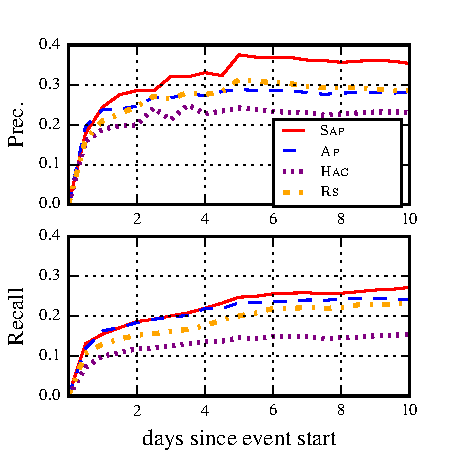
\includegraphics[scale=1.0]{feature_based_salience_models/figures/rouge-timev2.pdf}
   % \input{feature_based_salience_models/figures/rouge-timev2.eps_tex}
   % \input{feature_based_salience_models/figures/rouge-timev2.tex}
    \caption{System \rougeN{1} performance over time.}
\label{fig:3_aps_rouge_time}
\end{wrapfigure}


Of the 25 events in the TREC TS data, 24 are
covered by the news portion of the TREC KBA
Stream Corpus. From these 24, we set aside
three events to use as a development set. All
system salience and similarity threshold parameters
are tuned on the development set to maximize
\rougeN{2} \fmeasure{} scores.
We train a salience model for each event using
1000 sentences randomly sampled from the
event's document stream.
We perform a leave-one-out evaluation of each
event. At test time, we predict a sentence’s
salience using the average predictions of the 23
other models.



    Since we lacked gold judgements about what sentences contain which nuggets
    we perform an automatic evaluation using \rouge{} \citep{lin2004rouge}. We 
    create reference summaries for each query by concatenating all 
    of it's nugget texts.
    Since there are no fixed summary lengths, and depending on the severity
    of the event, the reference summaries can vary greatly in length.
    To account for this, we report \rouge{} recall, precision and \fmeasure{}
    score.
We also approximate the manual evaluation of the official TREC TS track
    by automatically mapping sentences to nuggets if their semantic similarity
    is a above a threshold. 
    We report $\expectedGain,$ $\comp,$ and their \fmeasure{} score
    across a sweep of similarity threshold 
    values from zero to one, with values closer to one a more conservative
    estimate of performance.     


    We refer to our approach as \sap{} and compare to 
    several 
    baselines.
    The first is our full system but with uniform salience scores, i.e.
    the default AP clustering algorithm. We refer to
    this method as \ap.
    The second is to rank all sentences in each batch in order of decreasing
    predicted
    salience, and sequentially adding each sentence to the update summary, 
    omitting
    any sentences with similarity to previous updates above a threshold.
    This method is referred to as \ranksal{} for rank by salience.
    Finally, we compare against another clustering algorithm,
    hierarchical agglomerative clustering.
    In this method, sentences are first clustered, 
    and then centers are determined by the sentence
    with  highest  cosine  similarity  to  the  cluster
    mean. 
    Sentences are added to the update summary in time order, 
    removing sentences that are highly similarity to previous updates in the
    same manor as the \ranksal{} method. We refer to this method as 
    \hac.



\begin{wrapfigure}{R}{0.45\textwidth}
 \center
 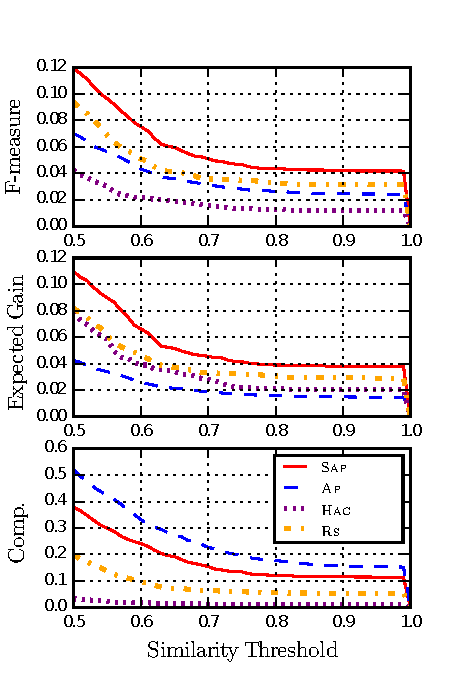
\includegraphics[scale=1.0]{feature_based_salience_models/figures/nuggets-metrics3.pdf}
 \caption{Expected Gain and Comprehensiveness performance.}
 \label{fig:3_aps_autots}
\end{wrapfigure}


    \subsubsection{Results}

\autoref{tab:aps_rouge}  shows  our  results  for  system  output
samples against the full summary of nuggets using \rouge. 
This improvement is statistically significant  for  all  ngram  
precision,  recall,  and \fmeasure{} scores at the
$\alpha=.01$
level using the Wilcoxon
signed-rank test.
\sap{}
maintains    its    performance
above  the  baselines  over  time  as  well.
\autoref{fig:3_aps_rouge_time}  shows  the  \rougeN{1}  scores  over  
time.
We  show  the  difference  in  unigram  precision
(bigram  precision  is  not  shown  but  it  follows a
similar  curve).
Within  the  initial  days  of  the
event,  \sap{}
is  able  to  take  the  lead
over  the  over  systems  in  ngram  precision.   The
\sap{}
model is better able to find salient
updates earlier on; for the disaster domain, this is
an especially important quality of the model.
Moreover, the \sap{} recall is not diminished by the high 
precision and remains competitive with \ap. 
Over time \sap's recall also begins to pull away, 
while the other models start to suffer from topic drift.


\autoref{fig:3_aps_autots} shows the $\expectedGain$ and $\comp$
across a range
of  similarity  thresholds,  where  thresholds  closer
to 1 are more conservative estimates. The ranking
of the systems remains constant across the sweep
with \sap{}
beating all baseline systems.
Predicting salience in general is helpful for keeping a summary on topic as 
the  \ranksal{}  approach out
performs  the  clustering  only  approaches  on  $\expectedGain$.
When looking at the $\comp$ of the
summaries \ap{} outperforms \sap.  
The compromise  encoded  in  the  \sap{}
objective function, between being representative and
being salient, is seen clearly here where the performance of the \sap{}
methods is lower
bounded by the salience focused  \ranksal{}  system and
upper bounded by the clustering only AP system.
Overall, \sap{}
achieves the best balance
of these two metrics.



\subsection{Model 2: Learning-to-Summarize}

The \sap{} model has two primary shortcomings on the stream summarization
task. First, by processing sentences in hourly batches, we potentially 
incur latency penalties if important information enters the stream
at the start of the hour.
Ideally we would process new documents as soon as possible in order 
to minimize the negative effects of latency. Second, the salience
regressors were statically trained without exploration. If we had 
some sort of exploration during training, we could take advantage of 
features between previous sentence selection decisions and the current
state of the update summary (something we didn't model in \sap).

In order to train with exploration, we need either many possible trajectories
(i.e. document streams and associated sentence extraction labels) for all
of the plausibly good summaries or some tractable oracle summarizer 
that we can use to complete a trajectory from any partially completed prefix
of extraction decisions. Since we lack even one ground truth trajectory, we
opt to use an oracle summarizer, which we refer to as the oracle policy, 
in keeping with the learning-to-search literature.



%Getting around these limitations poses some severe challenges. Using
%dynamic features means that naive training will require gold reference
%sentence extract sequences and that naively training a sentence salience model
%with these will under explore the space of plausable update summaries,
%meaning that at test time errors are likely to snowball over time.

The oracle policy $\oraclePolicy$ has knowledge of what nuggets, 
if any, are present in each sentence in the document stream, and it's behavior
is quite simple: it processes the document stream sequentially and when it 
encounters a sentence with a novel nugget, it adds that sentence to the update
summary.


As we stated before, training only on a single oracle run over document stream
would be sub-optimal because the oracle is perfect and it would finish 
recovering all of the nuggets quite quickly and then do nothing for
the remainder of the stream. In practice, our learned model is likely to
make mistakes, missing the first few appearances of a nugget but hopefully
recovering them as repetition in the stream makes them more likely to be 
selected. Only following the oracle's first best pass would not help us learn
to recover from errors.

To make better use of the oracle, we adopt the locally optimal learning to
search (LOLS) regime \citep{chang2015learning}, one of a family of 
learning-to-search algorithms. In order to formally describe the algorithm, we
first introduce some notation. We define the stream summarization task as a 
Markov decision process. We observe a sequence of states $\lsState_\lsStep \in 
\lsStateSpace$ which correpsond to observing the first $\lsStep$ sentences in 
the stream along with the first $\lsStep-1$ extraction decisions. A policy 
$\policy \in \policySpace$ maps states to
actions where the action space $\lsActionSpace = \{\lsAction_0, \lsAction_1\}$ contains two 
actions with $\lsAction_0$ indicating ``skip the current sentence'' and 
$\lsAction_1$ 
indicating ``extract the current sentence.'' 
Transitions between states are deterministic, i.e. the $\lsStep$-th 
sentence in the stream is appended to the update summary if $\lsAction_1$
was selected and the next stream sentence is presented to the summarizer.
%A deterministic transition
%function $\fdef{\lsTrans}{\lsStateSpace \times \lsActionSpace}{\lsStateSpace}$.
%maps state-action pairs $(\lsState_\lsStep, \lsAction_\lsStep)$ to the next 
%state $\lsState_{\lsStep + 1}$, i.e. updating the observed
%sentences with the next, i.e. $(\lsStep + 1)$-th, sentence from the stream 
%and 
%updating the prefix of extraction variables with $\lsAction_\lsStep$.
A trajectory $(\lsState_1, \lsAction_1), \ldots, (\lsState_n, \lsAction_n)$
of state-action tuples
implicitly defines an extract label sequence $\lsSaliences \in \{0, 1\}^n$
for a stream of $n$ sentences.
Additionally, we assume possession of a non-negative loss function 
$\lsStrucLoss(\lsSaliences, \lsSaliencesRef)$
which measures the discrepancy between the predicted extract sequence 
$\lsSaliences$ and a reference sequence $\lsSaliencesRef$.
The model policy interacts with states through a feature
map $\fdef{\lsFeats}{\lsStateSpace}{\Rn{d}}$ and a matrix 
of associated feature
weights $\policyParams\in \Rn{2 \times d}$ via $\policy(\lsState_\lsStep)
= \operatorname{arg\; min}_{\lsAction \in \lsActionSpace} 
    \policyParams_\lsAction \cdot \lsFeats(\lsState_\lsStep)$.


In the LOLS regime, model training works by exploring the state space in 
two phases. Consider a case where the document stream consists of $n$ 
sentences. The first phase, called 
the \textit{roll-in}, uses the current model policy $\modelPolicy$ (which
is initially random) to explore $\lsStep$ steps into the stream, i.e. starting
from state $\lsState_1$, we repeatly apply $\modelPolicy$ and take it's 
predicted action, stopping at state $\lsState_\lsStep$. 
In the second phase we complete the trajectory using either the oracle 
$\oraclePolicy$ or $\modelPolicy$ (the probability $\lsChoiceParam$ of using 
$\oraclePolicy$ over $\modelPolicy$ is a hyperparameter). Let 
$\rollOutPolicy$ be the roll-out policy, and let 
$\lsSaliencesRollOut^{(\lsState_\lsStep, \lsAction)}$ be the extract label
sequence implied by the completed trajectory of using $\modelPolicy$
to navigate to $\lsState_\lsStep$, taking action $\lsAction$, 
and then using $\rollOutPolicy$ to complete the trajectory from 
$\lsState_{\lsStep + 1}$.

We also associate with $\lsSaliencesRollOut^{(\lsState_\lsStep, \lsAction)}$
a non-negative cost $\lsCost(\lsState_\lsStep, \lsAction)$ which connects 
the global discrepancy of the resulting structured loss to the local action
decisions via the following formula
\[
    \lsCost(\lsState_\lsStep, \lsAction) = 
      \max_{\lsAction^\prime \in \lsActionSpace}
        \lsStrucLoss(
            \lsSaliencesRollOut^{(\lsState_\lsStep, \lsAction)},
            \lsSaliencesRef)
        - 
        \lsStrucLoss(
            \lsSaliencesRollOut^{(\lsState_\lsStep, \lsAction^\prime)},
            \lsSaliencesRef).
\]
The cost of the locally optimal action will be zero, while the 
the locally sub-optimal action will have a cost equal to the difference
between the structured losses associated with the sub-optimal and optimal 
actions as completed by $\rollOutPolicy$.

For each epoch of training, we select a training stream and for 
each sentence in the stream we perform a roll-in/roll-out, collecting
the associated costs at each step into a dataset
$\dataset = \big\{\big(\lsFeats(\lsState_1), \lsCost(\lsState_1, \lsAction_0), \lsAction_0\big), \ldots,
\big(\lsFeats(\lsState_T), \lsCost(\lsState_T, \lsAction_1), \lsAction_1\big) \big\}$.
After computing all costs for a given
stream $\strsents(\query)$, we update $\modelPolicy$ to minimize the mean
squared error of the sampled costs, i.e. we minimize the function
\[ 
  %  \objective\big(\policyParams, \strsents(\query)\big) =
    \objective(\policyParams) =
    \frac{1}{|\dataset|} \sum_{\lsFeats(\lsState_\lsStep), \lsCost(\lsState_\lsStep, \lsAction), \lsAction \in \dataset}  
\Big( \lsCost(\lsState_\lsStep, \lsAction) -  \policyParams_{\lsAction} \cdot \lsFeats(\lsState_\lsStep, \lsAction) \Big)^2 \]
using stochastic gradient descent. 

%\begin{figure}
 \begin{algorithmic}[1]
  \Procedure{LolsTraining}{}
   \State Randomly initialize $\policyParams$.
   \Repeat
    \For{$\query \in \Queries$}
     \State $\dataset \gets \varnothing$
     \For{$\lsStep = 1, \ldots, T$}
        \State Roll-in by executing $\modelPolicy$ for $\lsStep$ steps to 
arrive at state $\lsState_\lsStep$.
        \State Set roll-out policy $\rollOutPolicy = \oraclePolicy$ with probability $\lsChoiceParam$, otherwise $\modelPolicy$.
       \For{$\lsAction \in \lsActionSpace$}
            \State Use $\rollOutPolicy$ to complete trajectory to obtain cost
            $\lsCost(\lsState_\lsStep, \lsAction)$
            \State $\dataset \gets \dataset \cup \{ 
            \big(\lsFeats(\lsState_\lsStep), 
        \lsCost(\lsState_\lsStep, \lsAction), \lsAction \big) \}$
        
       \EndFor
     \EndFor
     \State $\policyParams = \policyParams - \gamma \nabla\objective(\policyParams)$
    \EndFor
   \Until{convergence}
  \EndProcedure
 \end{algorithmic}
 \caption{The locally optimal learning to search (LOLS) training algorithm.
 $\gamma$ is a learning rate.}
 \label{alg:lols}
\end{figure}


See \cite{kedzie2016real} for the full LOLS training algorithm.
The benefit of using $\modelPolicy$ to obtain the roll-in trajectory 
is that the oberved state spaces are more likely to be similar to ones visited
on test data since compounding error in $\modelPolicy$ will also effect the 
states visited at training 
time and thus minimizing train/test distribution mismatch. 
Randomly selecting $\oraclePolicy$ versus $\modelPolicy$ is similarly 
helpful for ensuring that the completed trajectory is somewhat realistic
(i.e. when using $\modelPolicy$) but can also learn the behavior 
of the more perfect oracle. The theoretical motivations of LOLS can be found
in greater depth in \cite{chang2015learning}.


\subsubsection{Oracle Policy and Loss Function}

We use a greedy oracle that selects sentences that contain novel
nuggets. This oracle will achieve an optimal \comp{} score, i.e.
it will obtain every possible novel nugget in the roll-out phase.
%However, it will not always achieve the maximum possible $\expectedGain$.
%For example, consider the sequence of sentences $s_1, s_2, s_3$, where
%nugget $n_1 \in s_1$, $n_2 \in s_2$, and $n_1,n_2 \in s_3$. The greedy oracle,
%proceeding sequentially would select sentences $s_1$ and $s_2$, and skip
%$s_3$, achieving an $\expectedGain$ of $\frac{|\{n_1, n_2\}|}{|\{s_1, s_2 \}|}
%= \frac{2}{2} = 1$. The maximum achievable $\expectedGain$ is obtained by 
%skipping
%the first two sentences and selecting sentence $s_3$ yielding $\frac{|\{n_1, n_2\}|}{|\{s_3 \}|} = \frac{2}{1} = 2$. In practice we are far from matching
%the greedy oracle and so it suffices for now as an aspirational target.
In order to implement a loss function $\lsStrucLoss$ we need a reference
extract label sequence $\lsSaliencesRef$ for which to compare to the one 
obtained by the model policy, $\predSaliences$. We set 
$\lsSaliencesRef_\lsStep = 1$ if the oracle policy would have selected that
sentence given the prefix of predicted extractions $\predSaliences_{1:\lsStep -1}$, i.e. if the $\lsStep$-th sentence contained a nugget not contained in
any previous sentence extracted by $\modelPolicy$, the reference extract would
contain it.

We design our loss function to penalize policies that severely over- or
 under-generate. 
 Given the reference and predicted extract summaries, 
 we define the loss as the complement of
 the Dice coefficient between the decisions,
\begin{align*}
  \lsStrucLoss(\lsSaliencesRef, \predSaliences) = 1 - 2 \times 
    \frac{ \sum_i \lsSaliencesRef_i \predSaliences_i }{ 
    \sum_i \lsSaliencesRef_i + \predSaliences_i }.
\end{align*}

 This encourages not only local agreement between policies (the numerator of
 the second term) but that the learned and oracle policy should generate
 roughly the same number of updates (the denominator in the second term).

\subsubsection{Salience Estimation}
The model policy accesses a state-action tuple through the feature function 
$\lsFeats$, upon which we learn a linear function of the features to predict 
the anticipated cost of skipping or extracting the sentence. We can interpret
the negative cost of selecting a sentence as its salience to the event
query. Since a
state $\lsState_\lsStep$ encodes the first $\lsStep$ sentences and $\lsStep-1$
extraction decisions made while processing the document stream, $\lsFeats$
can represent a broader range of features than a salience model trained 
on static sentence salience judgements. In particular, we have several
similarity features between the current sentence under consideration and
the current state of the update summary. See \autoref{sec:features} for the 
complete list of features. 

Many of our features are helpful for
 determining the importance of a sentence with respect to its document.
 However, they are more ambiguous for determining importance to the event as
 a whole. %For example, it is not clear how to compare the document level
% PageRank of sentences from different documents. 
 To compensate for this, we
 leverage two features which we believe to be good global indicators of
 update selection: the summary content probability and the document
 frequency.  These two features are proxies for detecting (1) a good summary
 sentences (regardless of novelty with respect to other previous decisions)
 and (2) when an event is likely to be producing novel content. 
 Therefore, we also 
 compute
  feature conjunctions of all features in \autoref{sec:features} with the nugget 
 probability and document 
 frequency separately, as well as together.

\subsubsection{Data}
We used the official TREC 2015 Temporal Summarization dataset which 
was expanded from the previous year (on which we evaluated the \sap{} model).
We use an expanded version of the stream corpus used in \autoref{sec:sapmodel}
collected by \cite{frank2012building}. 
The event query dataset was also expanded to 44 total queries with coverage 
in the stream stream corpus. Nuggets for the additional events were also 
collected. Additionally, pooled output from the 2015 TS performer submissions
was manually labeled by NIST to obtain nugget relevance judgements. We used 
these judgements to build the nugget probability feature 
%(see \autoref{par:nuggetprob}) 
and to add noisy labels to the corpus.
 

 Because of the large size of the corpus and the limited size of the manual
 annotation pool,
 many good candidate sentences were not manually reviewed.
 Less than 1\% of the sentences in our relevant document streams received
 manual review.  In order to increase the amount of data for training and
 evaluation of our system, we augmented the manual judgements with automatic
 or ``soft'' matches. A separate gradient boosting classifier was trained for
 each nugget with more than 10 manual sentence matches.  Manually matched
 sentences were used as positive training data and an equal number of
 manually judged non-matching sentences were used as negative examples.
 Ngrams (1-5), percentage of nugget terms covered by the sentence,
 semantic similarity of the sentence to nugget were used as features, along
 with an interaction term between the semantic similarity and coverage. When
 augmenting the relevance judgments with these nugget match soft labels, we
 only include those that have a probability greater than 90\% under the
 classifier. Overall these additional labels increase the number of matched
 sentences by 1600\%.
 
% For evaluation, the summarization system only has access to the query and
% the document stream, without knowledge of any nugget matches (manual or
% automatic).





%~\\~\\
%
%While our learning objective is to minimize the expected 
%structured loss $\lsStrucLoss$,
%the model policy makes greedy local local actions. We use a cost function 
%over state-action pairs to connect the global structure discrepancy to
%local action choices by defining the cost function as 
%%$\fdef{\lsCost}{\lsStateSpace\times\lsActionSpace}{\Rnonneg}$
%\[
%    \lsCost(\lsState, \lsAction)
%\]
%
%
%and update a cost-sensitive 
%classifier to predict the 
%
%
%
%~\\
%
%We treat the streaming summarization problem
%as a Markov decision process. At each timestep $t$ we observe a state
%$s_t \in \mathcal{S}$ and $t$-th sentence $x_t \in \mathcal{X}$ from the 
%document stream.
%A policy $\pi : \mathcal{S} \times \mathcal{X} \rightarrow \{0, 1\}$
%maps a state-sentence tuple to an action $a \in \mathcal{A} =\{0,1\}$
%where $a=1$ indicates we extract the sentence and $a=0$ indicates we skip
%the current sentence. The transition function 
%$d : \mathcal{S} \times \mathcal{X} \times \mathcal{A} \rightarrow \mathcal{S}$
%deterministically maps state-sentence-action tuples to the next state. 
%In practice the state contains set of sentences previously extracted and
%other rolling statistics from previously observed sentences in the stream.
%Our training objective is to minimize the expected costs of each action:
%\[ \mathcal{L}(\pi) = \mathbb{E}_{s,x \sim \pi} \left[ c\left(\pi(s,x), s, x\right) \right] \]
%where $c :\mathcal{A} \times \mathcal{S} \times \mathcal{X} \rightarrow \mathcal{A}$ is the cost of taking a given action in a particular state-sentence
%observation.
%
%~\\
%
%~\\
%
%In the LOLS training regime, there are two phases: the 
%\emph{roll-in} and the \emph{roll-out}. The roll-in phase 
%
%at each timestep 
%we alternate between using the oracle $pi^o$ or our current learned policy
%$\hat{\pi}$ to run multiple time steps into the future and get a cost for 
%a hypothetical summary we would have created in the case where we extracted the 
%current sentence or skipped it. We collect these scores for each decision
%and update a regression model to accuractely predict the cost of each action
%given the current sentence and update summary/stream state.
%
%





\subsubsection{Experiments }

 To evaluate our model, we randomly select five events to use as a
 development set and then perform a leave-one-out style evaluation on the
 remaining 39 events.
 Even after filtering,  each training query's document stream is still too
 large to be used directly in our combinatorial search space. In order to
 make training time reasonable yet representative, we downsample each stream
 to a length of 100 sentences. The downsampling is done uniformly over the
 entire stream. This is repeated 10 times for each training event to create a
 total of 380 training streams. In the event that a downsample contains no
 nuggets (either human or automatically labeled) we resample until at least
 one exists in the sample. 

 In order to avoid overfitting, we select the model iteration for each
 training fold based on its performance (in F-measure of $\expectedGain$ and
 $\comp$) on the development set.


 We refer to our ``learning to summarize'' model in the results as 
 \modelLS.
 We compare our proposed model against several baselines and extensions. 

 %\paragraph{Cosine Similarity Threshold} 
 One of the top performing systems 
 at TREC 2015 was a heuristic method that only
 examined article first sentences, selecting those that were below a cosine
 similarity threshold to any of the previously selected updates. We
 implemented a variant of that approach using the latent-vector
 representation used throughout this work \citep{guo2012simple}. 
 The development set was used to
 set the threshold. We refer to this model as \modelCos{} (Team
 \textsc{WaterlooClarke} at TREC 2015).
  
% \paragraph{Salience-biased Affinity Propagation}
 We also compare this model to a simplified varient of the \sap{} model
where we use the summary
nugget probability feature as the salience estimator (the Gaussian process
models were difficult to scale to the expanded dataset).  The time
 window size, similarity threshold, and an offset for the cluster preference
 are tuned on the development set.
 As in the \modelCos{} model, a
 similarity threshold is used to filter out updates that are too similar to
 previous updates (i.e. previous clustering outputs).    
 We refer to this method as \sap.  

 %\paragraph{Learning2Search+Cosine Similarity Threshold} 
 Our final baseline, which we
 refer to as \modelLSCos, we run \modelLS{} as before, but filter the
 resulting updates using the same cosine similarity threshold method as in
 \modelCos. The threshold was also tuned on the development set. 


 \subsubsection{Results}
 \begin{figure*}
    \center
\begin{tabular}{ l | l l l | l l l | l }
   &\multicolumn{3}{c|}{unpenalized}&\multicolumn{3}{c|}{latency-penalized}&\\
   & exp. gain     & comp. & $F_1$ & exp. gain     & comp. & $F_1$ & num. updates\\
    \hline
%\textsc{AP}         
%    & $0.083$            & $0.09$                     & $0.078$ 
%    & $0.079$            & $0.095$                    & $0.077$ 
%    & ~~$20.846^{s}$ \\
\sap      
    & $\mathbf{0.119}^c$ & $0.09$                     & $0.094$ 
    & $0.105$            & $0.088$                    & $0.088$ 
    & ~~~~$8.333$ \\
\modelCos
    & $0.075$            & $0.176^{s}$              & $0.099$ 
    & $0.095$            & $0.236^{s}$              & $0.128^{s}$ 
    & $145.615^{s,f}$ \\
\modelLS       
    & $0.097$            & $\mathbf{0.207}^{s,f}$   & $0.112$ 
    & $0.136^{c}$      & $\mathbf{0.306}^{s,c,f}$ & $0.162^{s}$
    & ~~$89.872^{s,f}$ \\
\modelLSCos
    & $0.115^{c,l}$        & $0.189^{s}$ & ${\bf0.127}^{s,c,l}$
    & ${\bf0.162}^{s,c,l}$ & $0.276^{s}$ & ${\bf0.184}^{s,c,l}$
 & ~~$29.231^{s,c}$ \\
\end{tabular}
\caption{
 Average system performance 
 and average number of updates per event.
 Superscripts indicate significant improvements ($p < 0.05$) between the run and
 competing algorithms using the 
  paired randomization test with the Bonferroni correction for multiple 
  comparisons ($s$: \sap, 
 $c$: \modelCos, $l$: \modelLS, $f$: \modelLSCos). 
}
\label{fig:lsresults}
\end{figure*}


  Results for system runs are shown in \autoref{fig:lsresults}.  On average,
  \modelLS{} and \modelLSCos{} achieve higher \fmeasure{} scores than the baseline
 systems in both latency penalized and unpenalized evaluations. For
 \modelLSCos, the difference in mean \fmeasure{} score was significant compared
 to all other systems (for both latency settings).
 
 \sap{} achieved the overall highest $\expectedGain$, partially because
 it was the tersest system we evaluated. However, only \modelCos{} was
 statistically significantly worse than it on this measure. %Interestingly,
 
 In comprehensiveness, \modelLS{} recalls on average a fifth of the nuggets
 for each event. This is even more impressive when  compared to the average
 number of updates produced by each system (\autoref{fig:lsresults}); while
 \modelCos{} achieves similar comprehensiveness, it takes on average about
 62\% more updates than \modelLS{} and almost 400\% more updates than
 \modelLSCos. The output size of \modelCos{} stretches the limit of the
 term ``summary,'' which is typically shorter than 145 sentences in length.
 This is especially important if the intended application is negatively
 affected by verbosity (e.g. crisis monitoring).

 \begin{figure}
  \center
  \begin{tabular}{ l | l l l |}
    &\multicolumn{3}{c}{latency-penalized}\\
    & exp. gain     & comp. & $F_1$ \\
    \hline
    \small \modelCos{}  & $0.095$ & $\mathbf{0.236}$ & $0.128$ \\
    \small \textsc{LS-FS}  & $0.164$ & $0.220$ & $0.157$ \\
    \small \textsc{LS-Cos-FS} & 
      $\mathbf{0.207}$ & $0.18~~$ & $\mathbf{0.163}$ \\
  \end{tabular}
  \caption{Average system performance. \textsc{LS-FS} and \textsc{LS-Cos-FS} 
           runs are trained and evaluated on first sentences only (like the 
           \textsc{Cos} system). Unpenalized results are omitted for space but
           the rankings are consistent.}
  \label{fig:lsfsresults}
\end{figure}




 Since \modelCos{} only considers the first sentence of each document, it
 may miss relevant sentences below the article's lead. In order to confirm the
 importance of modeling the oracle, we also trained and evaluated the
 \modelLS{} based approaches on first sentence only streams. Figure
 \ref{fig:lsfsresults} shows the latency penalized results of the first
 sentence only runs.  The \modelLS{} approaches still dominate \modelCos{}
 and receive larger positive effects from the latency penalty despite also
 being restricted to the first sentence. Clearly having a model (beyond
 similarity) of what to select is helpful. Ultimately we do much better when
 we can look at the whole document.
  
% \begin{figure}
  \center
  \begin{tabular}{l|l|l|l|l|l}
    & Miss  &      Miss  &          &    &  \\
    & Lead &      Body &         Empty &   Dupl. & Total \\
    \hline
    \small \sap{}      
      & 29.6\% & 68.7\% & ~~1.6\% & 0.1\% & 15,986\\
    \small \modelCos     
      & 17.8\% & 39.4\% & 41.1\% & 1.7\% & 12,873\\
    \small \textsc{LS-FS}      
      & 25.4\% & 71.7\% & ~~2.0\% & 0.9\% & 13,088\\
    \small \textsc{LS-Cos-FS}
      & 27.9\% & 70.8\% & ~~1.0\% & 0.2\% & 15,756\\
    \small \modelLS{}           
      & 19.6\% & 55.3\% & 19.9\% & 5.1\% & 13,380\\
    \small \textsc{LS-Cos}    
      & 24.6\% & 66.7\% & ~~7.5\% & 1.2\% & 11,613\\
  \end{tabular}
  \caption{Percent of errors made and total errors on test set.}
  \label{fig:lserrors}
\end{figure}

%
%  We also performed an error analysis to further understand how each system
% operates.  \autoref{fig:lserrors} shows the errors made by each system on
% the test streams.  Errors were broken down into four categories. \emph{Miss
% lead} and \emph{miss body} errors occur when a system skips a sentence
% containing a novel nugget in the lead or article body respectively. An
% \emph{empty} error indicates an update was selected that contained no nugget.
% \emph{Duplicate} errors occur when an update contains nuggets but none are
% novel. 
% 
%  Overall, errors of the miss type are most common and suggest future
% development effort should focus on summary content identification.  About a
% fifth to a third of all system error comes from missing content in the lead
% sentence alone.
% 
%  After misses, empty errors (false positives) are the next largest source of
%  error. \modelCos{} was especially prone to empty errors (41\% of its total
%  errors). \modelLS{} is also vulnerable to empties (19.9\%) but after
% applying the similarity filter and restriting to first sentences, these
% errors can be reduced dramatically (to 1\%).
%  
%  Surprisingly, duplicate errors are a minor issue in our evaluation. This is
% not to suggest we should ignore this component, however, as efforts to
% increase recall (reduce miss errors) are likely to require more robust
% redundancy detection. 




\section{Deep Learning Models of Word and Sentence Salience}

\label{sec:chapter4}

\def\tfidf{TF-IDF}

Estimating the salience of words and phrases is core to the problem of 
summarization. For example, \cite{luhn1958automatic} 
noted how the most topically central words in a document occur not too much 
but not
too little, and that,
``the presence in the region of highest frequency of many of the words
 previously described as too common to have the  type  of
 significance being sought would constitute
`noise' in the system.''

Subsequently, many methods have been proposed for salience estimation
in the context of summarization. Word weights have typically been derived
in an unsupervised way from a large collection of in-domain text.
The classic example here is Term Frequency-Inverse Document Frequency
(\tfidf) weighting \citep{sparck1972statistical}, whose aim is similar in 
spirit to Luhn's: important 
words occur frequently in the current context (the term frequency component)
 but not so much that they occur in every document 
(the inverse frequency component).

While \tfidf weights (and others like BM25 \citep{bm25}) have been frequent
ingredients in many summarization systems \citep{a,b,c,d,e}, they are 
not specifically tuned to any one summarization task. Another prominent
strand of research has been the learning of word or ngram specific weights
typically for use in linear models of salience \citep{martins2009summarization,woodsend2010automatic,berg2011jointly,durrett2016learning}. 
Given the small size of most summarization datasets at the time, one could question 
the utility of learning ngram weights when it was unlikely that there 
would be adequate data to learn broad coverage summarizers.

This 
situation has changed with the recent availability of large scale summarization data \citep{cnndm,newsroom,nyt}. With these corpora,
and other developments in word embedding representation \citep{miklov,glove},
many researchers have been developing end-to-end models of both 
abstractive \citep{abs} and extractive \citep{ext} summarization.
While the spirit of ``let a thousand architectures bloom'' has spurred much
creativity and performance gains, it has left us with little explainability
about how such models work. 

While different components of the neural architectures may be justified 
by intuition, these methods are largely black boxes and it is not clear
how they are making their sentence selection predictions. This is especially
problematic in abstractive summarization, but it is also not well understood
how extractive methods make their decisions either.

In this chapter, we describe completed experiments teasing out the importance
of different neural network designs for sentence level salience. This
work describes impedements to learning and word and sentence representations
in deep learning models of extractive summarization, and led to 
a recent publication \citep{kedzie2018deep}. Based on these limitations,
we propose extensions to the word level representations and explicitly model
word level salience scores as a means to performing sentence extractive
summarization. While the finished and proposed work focuses on single document
summarization, we also propose an extension of the word level salience
estimation model that we hope will generalize to the multi-document
summarization context.


%In this chapter we investigate neural network architectures for extractive
%summarization, in the hopes of better understanding what is important 
%for the underlying word and sentence representations to learn.
%We start a description of completed experiments for sentence extractive
%models of summarization \citep{kedzie2018deep}, and then complete the chapter with a description
%of planned and ongoing word importance estimation techniques using deep
%learning models.


~~\\
~\\






Increasingly, researchers are returning to single document summarization,
once thought to be too difficult for automatic summarization methods.
This has been driven both by the availability of large corpora (the
most popular corpus, CNN-DailyMail, has a little over 300,000 data points
\citep{see2017get}) and by the development of general purpose 
generative models of text from the neural machine translation community.
Accordingly, the bulk of the research has used this corpus, (and the NYT
corpus \citep{sandhaus2008new}) to focus on abstractive summarization
research \citep{rush2015neural,chopra2016abstractive,cheng2016neural,nallapati2016abstractive,see2017get,paulus2017deep}. 
There has been a smaller but similar proliferation of sentence
extractive single document summarization papers on these corpora also using 
neural network architectures \citep{cheng2016neural,nallapati2016classify,nallapati2016abstractive,narayan2018ranking}.



\ifthenelse{\equal{\highlevel}{false}}{
  
\newcommand{\sent}{s}
\newcommand{\Sents}{\mathcal{S}}
\newcommand{\doc}{D}
\newcommand{\lbl}{y}
\newcommand{\Labels}{Y}
\newcommand{\word}{w}
\newcommand{\vocab}{\mathcal{V}}
\newcommand{\extracts}{\mathcal{E}}
\newcommand{\budget}{c}
\newcommand{\encoder}{\textsc{Encoder}}
\newcommand{\extractor}{\textsc{Extractor}}
\newcommand{\embproj}{W}
\newcommand{\emb}{\omega}
\newcommand{\embsize}{n}
\newcommand{\sembsize}{m}
\newcommand{\semb}{h}
\newcommand{\rsemb}{\overrightarrow{\semb}}
\newcommand{\lsemb}{\overleftarrow{\semb}}
\newcommand{\gru}{\textsc{Gru}}
\newcommand{\rgru}{\overrightarrow{\gru}}
\newcommand{\lgru}{\overleftarrow{\gru}}
\newcommand{\cfeat}[2]{f_{#1}^{( #2 )}}
\newcommand{\relu}{\textsc{ReLU}}
\newcommand{\winsize}{k}
\newcommand{\winsizes}{K}
\newcommand{\fmapsize}{F}
\newcommand{\cfidx}{l}
\newcommand{\cact}{a^{(\cfidx,\winsize)}}
\newcommand{\cnnbias}{u^{(\winsize)}}
\newcommand{\cnnweight}{U^{(\winsize)}}
\newcommand{\cnnBiasSpace}{\mathbb{R}^{\fmapsize_\winsize}}
\newcommand{\cnnWeightSpace}{\mathbb{R}^{\winsize \times \fmapsize_\winsize \times \embsize}}


\subsection{Deep Learning Models of Sentence Extraction}

 Given the diversity of neural architectural choices, a best practices
for sentence extracive summarization has yet to emerge. In this section
we ask what architecture design choices matter for single document 
summarization across a variety of domains.

We begin by definining some terminology. A sentence is represented as an
sequence of words $\sent = \{\word_1, \word_2, \ldots, \word_{|\sent|} \}$
where each word is drawn from a fixed vocabulary $\vocab$ and $|\sent|$ is
the length of sentence $\sent$ in words. Similarly, a document $\doc = \{ 
\sent_1, \sent_2, \ldots, \sent_{|\doc|} \}$ is a sequence of sentences, where 
$|\doc|$ is the size of the document in sentences.  

We treat the sentence extractive summarization as sequence tagging
problem: given a document $\doc$, we want to assign an associated binary
tag sequence $\Labels = \{\lbl_1, \lbl_2, \ldots, \lbl_d \}
\in \{0,1\}^d$ such that the extract summary $\extracts = \{ 
\sent_i \in \doc : \lbl_i =1 \}$ implied by $\Labels$ is a suitable summary
of the document. Typically, it is assumed that size of the extract summary
$|\extracts| = \sum_{i=1}^{|\doc|} \mathbbm{1}\{\lbl_i =1 \} \ll |\doc|$.
It is also common to enforce a word budget $\budget$ such that
$\sum_{\sent \in \extracts} |\sent| \le \budget$.

A typical deep learning model will build up a hierarchical representation
of each sentence, starting at the word level, and then composing an arbitrarily
long sequence of word representations into a fixed length sentence 
representation.
First the individual words are 
projected to fixed length vectors, or word embeddings via a mapping
$\embproj : \vocab
\rightarrow \mathbb{R}^{\embsize}$. The sentence encoder network $\encoder :
\{\mathbb{R}^{\embsize}\}^* \rightarrow \mathbb{R}^{\sembsize}$ is then 
responsible for mapping word embbeding sequences to fixed length sentence 
embeddings. Finally, the sentence extractor network $\extractor : 
\{\mathbb{R}^\sembsize\}^* \rightarrow \{0, 1\}^*$ produces a label 
sequence $\Labels$.

We explore several choices of encoder and extractor architecture from the 
literature \citep{cheng2016neural,nallapati2016summarunner} as well as 
propose our own designs \citep{kedzie2018deep}. In the next sections,
we describe the three sentence encoder architectures (\textit{avg}, 
\textit{rnn}, and \textit{cnn}) followed by four extractor architectures 
(\textit{rnn}, \textit{seq2seq}, \textit{sr}, and \textit{cl}).

\subsubsection{Sentence Encoders}
\paragraph{Averaging} The simplest encoder simply averages a sentence's
associated word embeddings:
\[ \encoder_{avg}(\sent) = \frac{1}{|\sent|} \sum_{\word \in \sent} \embproj(\word). \]
Other than the word embeddings, this encoder involves no learned parameters,
and while it collapses word order, embedding averaging has consistently
been found competitive with more sophisticated sentence embedding techniques
\citep{iyyer2015deep,wieting2015towards,arora2016simple,wieting2017revisiting}.


\paragraph{Recurrent Neural Networks} The second encoder architecture
we experiment with is a recurrent neural network (RNN) over the word
embeddings. An RNN maintains an internal ``hidden'' state that is sequentially
updated upon observing each word embedding. In practice, we use a bidirectional
RNN with a gated recurrent unit (GRU) as the particular instantiation of 
the RNN cell \citep{cho2014learning}.
Under the RNN encoder, a sentence embedding for a sentence $\sent$ is defined 
as
\begin{align}
\encoder_{rnn}(\sent) = [\overrightarrow{\semb}_{|\sent|}, \overleftarrow{\semb}_{1} ] & \\
  \rsemb_0 = \mathbf{0};& \quad 
  \rsemb_i = \rgru\left(\embproj(\word_i), \rsemb_{i-1}\right) \\
  \lsemb_{|\sent| + 1} = \mathbf{0};& \quad 
  \lsemb_i = \lgru\left(\embproj(\word_i), \lsemb_{i+1}\right) 
\end{align}
where $[\cdot]$ is the concatenation operator; $\rsemb_i$ and $\lsemb_i$ are
hidden states of the forward and backward GRU cells respectively; and 
$\rgru, \lgru : \mathbb{R}^\embsize \times \mathbb{R}^\sembsize 
\rightarrow \mathbb{R}^\sembsize$ are the forward and backward GRU cell 
operations.
\cite{nallapati2016summarunner} use a bidirectional RNN for their sentence
encoder.

\paragraph{Convolutional Neural Networks}
Our final sentence encoder uses a convolutional neural network
(CNN) to encode important ngram windows into a fixed length vector. 
CNN's have grown increasingly popular in many NLP tasks 
as a computationally efficient substitute for RNN-based architectures
\citep{kim2014convolutional,lei2015molding,dauphin2017language}.
Our architecture largely follows \cite{kim2014convolutional}: we apply a 
series of one dimensional convoluions over a sentence's word embeddings
using varying width convolutions. For each convolutional window size 
$\winsize \in \winsizes \subset \mathbb{N}$, a convolutional filter creates 
a feature vector $\cfeat{}{\winsize} \in \mathbb{R}^{\fmapsize_\winsize}$ 
and the encoder output is the concatenation of the $|\winsizes|$ vectors. 
The set of filter window sizes $\winsizes$ and the number of feature maps
$\fmapsize_\winsize$ for each $\winsize \in \winsizes$ are 
model hyperparameters.
Formally, we define the CNN encoding of a sentence $\sent$ as 
\begin{align}
\encoder_{cnn}(\sent) & = \left[\cfeat{}{\winsize} : \winsize \in \winsizes \right]\\
\cfeat{\cfidx}{\winsize} &= 
     \max_{i \in 1,\dots, |\sent| - \winsize + 1} 
       \relu\left(\cact_i \right) \\
\cact_i &= \cnnbias_\cfidx
    + \sum^{\winsize}_{j=1} \cnnweight_{\cfidx,j} \cdot \embproj(\word_{i + j -1})
\end{align}
where $\cnnbias \in \cnnBiasSpace$ and $\cnnweight \in \cnnWeightSpace$
are learned convolutional filter weights and $\relu(x) = \max(0, x)$ 
is the rectified linear unit \citep{nair2010rectified}. \cite{cheng2016neural}
uses a CNN for their sentence encoder.

\subsubsection{Sentence Extractors}

A sentence extractor takes the encoder output, i.e. 
a sequence of sentence embeddings
$\encoder(\doc) =$ $\{\encoder(\sent_1), \ldots, \encoder(\sent_{|\doc|})\} =
\{\semb_1, \ldots, \semb_{|\doc|}\}$, and produces a sequence of labels
$\Labels = \{\lbl_1, \ldots, \lbl_{|\doc|}\}$. 
The sentence extractor is essentially a discriminative
classifier $p(\lbl_1,\ldots,\lbl_{|\doc|} | \semb_1,\ldots,\semb_{|\doc|})$.
Previous neural network approaches to sentence extraction have assumed
an auto-regressive model, leading to a semi-Markovian
factorization of the extractor probabilities
$p(\lbl_{1:n}|\semb)=\prod_{i=1}^{|\doc|} 
p(\lbl_i|\lbl_{<i},\semb)$,
where each prediction $\lbl_i$ is dependent on \emph{all}
previous $\lbl_j$ for
all $j < i$. We compare two such models proposed by \cite{cheng2016neural}
and \cite{nallapati2017summarunner}.
A simpler approach that does not allow interaction among the $\lbl_{1:n}$
is to
%\hal{a simpler approach (explain why simpler) is a fully factored representation 
  model $p(\lbl_{1:n}|\semb) = \prod_{i=1}^n p(y_i|h)$,
  which we explore in two proposed extractor models that we refer to as the RNN 
  and Seq2Seq extractors.
%Implementation details for all extractors are in \autoref{app:sentextractors}.


%\paragraph{Previously Proposed Sentence Extractors}
% We consider two recent state-of-the-art extractors.
\paragraph{Cheng \& Lapata Extractor} 
 The first extractor we consider, proposed by 
\citet{cheng2016neural}, %, which we refer to as the Cheng \& Lapata Extractor,
is built around a sequence-to-sequence model.
First, each sentence embedding\footnote{\citet{cheng2016neural} used an CNN sentence encoder with 
this extractor architecture; in this work we pair the Cheng \& Lapata extractor
with several different encoders.} is
fed into an encoder side RNN, with the final encoder state passed to the
first step of the decoder RNN. On the decoder side, the same sentence 
embeddings are fed as input to the decoder and decoder outputs are used to
predict each $\lbl_i$. The decoder input is weighted by the previous extraction
probability, inducing the dependence of $\lbl_i$ on $\lbl_{<i}$.
See \autoref{fig:extractors}.c for a graphical layout of the extractor.
%and \autoref{app:clextractor} for details.

%?, but are delayed by one step and 
%?weighted by their prediction probability, i.e. at decoder step $t$,
%?$p(\slabel[t-1]|\slabel[<t-1], \sentEmb[<t-1]) \cdot \sentEmb[t-1]$\hal{why did you switch from $i$ to $t$?}
%?is fed into the decoder\hal{i don't udnerstand what this means. what op is $\cdot$?}. The decoder output at step $t$ is concatenated 
%?to the encoder output step $t$ and fed through a multi-layer perceptron
%?with one hidden layer and sigmoid unit output computing the $t$-th
%?extraction probability $p(\slabel[t]|\slabel[<t], \sentEmb[<t])$. \textcolor{red}{See Figure 2.c. for a graphical view. Full model details are presented in ??}.
%?

\paragraph{SummaRunner Extractor}\citet{nallapati2017summarunner} proposed
a sentence extractor, which we refer to as the SummaRunner Extractor,
that factorizes the extraction probability into contributions 
from different sources.
First, a bidirectional RNN is run over the sentence embeddings\footnote{\citet{nallapati2017summarunner}
    use an RNN sentence encoder with 
this extractor architecture; in this work we pair the SummaRunner extractor
with different encoders. } and the output is
concatenated. A representation of the whole document is made by 
averaging the RNN output. A summary representation is also constructed 
by taking the sum of the previous RNN outputs weighted by their extraction
probabilities. Extraction predictions are made using 
the RNN output at the $i$-th step, the document representation, and 
$i$-th version of the summary representation, along with factors for 
sentence location in the document. The use of the iteratively constructed
summary representation creates a dependence of $\lbl_i$ on all $\lbl_{<i}$.
See \autoref{fig:extractors}.d for a graphical layout.
%

%\paragraph{Proposed Sentence Extractors}
%We propose two sentence extractor models that 
%make a stronger conditional independence 
%assumption $p(\slabel|\sentEmb)=\prod_{i=1}^\docSize p(\slabel[i]|\sentEmb)$,
%essentially making independent predictions conditioned on $\sentEmb$.


\paragraph{$\extractor_{rnn}$}
    Our first proposed model is a very simple bidirectional
RNN based tagging model. As in the RNN sentence encoder we use a GRU cell.
The forward and backward outputs of each sentence are passed through a 
multi-layer perceptron with a logsitic sigmoid output 
to predict the probability
of extracting each sentence. 
See \autoref{fig:extractors}.a for a graphical layout.
%and \autoref{app:rnnextractor} for details.


\newcommand{\rExtHidden}{\overrightarrow{h}}
\newcommand{\lExtHidden}{\overrightarrow{h}}
\newcommand{\docSize}{|\doc|}
\newcommand{\logits}{o}

\begin{align}
    \rExtHidden_0 = \mathbf{0};&\quad   \rExtHidden_i = \rgru(\semb_i, \rExtHidden_{i-1}) \\
    \lExtHidden_{\docSize + 1} = \mathbf{0};&\quad    \lExtHidden_i = \lgru(\semb_i, \lExtHidden_{i+1}) \\
   \logits_i &= \relu\left(U \cdot [\rExtHidden_i; \lExtHidden_i] + u \right)\\
    p(\lbl_i=1|\encoder(\doc)) &= \sigma\left(V\cdot \logits_i + v  \right)
\end{align}
where $\rgru$ and $\lgru$ indicate the 
forward and backward GRUs respectively, and each have separate learned 
parameters; $U, V$ and $u, v$ are learned weight and bias parameters.
The hidden layer size of the GRU is 300 for each direction and the MLP hidden layer
size is 100. Dropout is applied to the GRUs and to $a_i$.





\paragraph{$\extractor_{s2s}$} One shortcoming of the RNN extractor is that long range
information from one end of the document may not easily be able to affect 
extraction probabilities of sentences at the other end. 
Our second proposed model, the $\extractor_{s2s}$ mitigates this problem with an 
attention 
mechanism commonly
used for neural machine translation \cite{bahdanau2014neural} and 
abstractive summarization \cite{see2017get}. 
The sentence embeddings are first
encoded by a bidirectional $\gru$. A separate decoder $\gru$ transforms each 
sentence into a query vector which attends to the encoder output. The
attention weighted encoder output and the decoder $\gru$ output are concatenated
and fed into a multi-layer perceptron to compute the extraction probability.
See \autoref{fig:extractors}.b for a graphical layout.




\subsection{Experiments}

 We are interested in two questions. The first, more pragmatic question, is
 what are the best configuration of encoder/extractor architectures?
 We answer this question by evaluating ROUGE recall and METEOR \citep{meteor}
 performance across our six collected datasets. We perform the standard
 stochastic gradient descent \cite{sgd} based optimization (using the Adam
 update \cite{adam}) of the weighted negative log likehood 
 \[ \mathcal{L}(\theta) = -\sum_{\Sents, \Labels \in \mathcal{D}} 
            \sum_i \omega(\lbl_i) 
        \log p(\lbl_i|\lbl_{<i}, \Sents; \theta) \]
        where $\theta$ are model parameters and $\omega(\lbl_i)$ upweights
        the positive labels to account for the imbalanced label distribution.

 We lack human reference extract labels for our datasets and so we obtain
 said lable sequences heuristically, by finding a label sequence $\Labels^*$
 by greedily optimizing ROUGE-1 recall with respect to the human reference
 abstracts.

 The second question, is more diagnostic in nature: what signals
 in the data are driving model learning?
 We perform several experiments to find answers. 
 We hypothesize that the lexical semantics encoded at the word embedding
 level will be important to subsequent sentence representations, and
 perform a comparison on learning with and with out fine tuning of the 
 embeddings. In both cases, embeddings are initialized with Glove
 embeddings pretrained on Wikipedia and Gigaword \citep{glove}.
 
 
 We also hypothesize that certain classes of words will be more important 
 to identifying salient content than others. We perform word ablation 
 experiments where we alternately remove nouns, verbs, adjectives \& adverbs,
 and function words from the sentence encoder input and compare performance 
 to the non-ablated system. We expect that the nouns will be more important
 to content selection. 


 Our final experiments attempt to tease out the effect of structural features 
 from the lexical. In this experiment, we shuffle the sentence order at 
 training time. In this setup, we obfuscate features about which content 
 was introduced in the article first, an important and well known bias in 
 news domain \cite{leadbias}. 


 \subsection{Results}


  

The results of our main experiment comparing 
the different extractors/encoders are shown in 
Table~\ref{tab:results}.
Overall, we find no major advantage when using the CNN and RNN sentence
encoders over the averaging encoder. The best performing encoder/extractor pair either 
uses the averaging 
encoder (five out of six datasets) or the differences 
are not statistically significant. %When only comparing within the 
%same extractor choice,  the averaging encoder is the better choice
%in 14 of 20 cases. 
%\hal{i wonder if it would be worth adding another ``average performance metric'' column to \autoref{tab:results}.
%  i'm thinking have ``Average $\Delta$-Best'' meaning how far (on average across the datasets) is this setting from the best setting available on that dataset.
%  so since the best numbers are: 25.56, 35.85, 23.11, 13.65, 5.63
%  and the first row numbers are: 25.42, 34.67, 22.65, 11.37, 5.50
%  then the deltas are:            0.14,  1.18,  0.46,  2.28, 0.13
%  the the average delta is 0.84 (assuming my math is right)
%  there's an argument to do multiplicative, in which case
%  the multipliers for first row:  0.99,  0.97,  0.98,  0.83, 0.97
%  and the average is 0.95
%  either way this gives a quick way to make comparisons between rows. you could do the same for the other tables too.}

  %\hal{in some of the tables you list R-2 as headers even though all the numbers are R-2. just put that in the caption.}


When looking at extractors, the Seq2Seq extractor is either part of 
the best performing system (three out of six datasets) or is not 
statistically distinguishable from the best extractor. 

Overall, on the news and medical journal domains, the differences are 
quite small with the 
differences between worst and best systems on the CNN/DM dataset 
spanning only .56 of a ROUGE point. While there is more performance variability
 in the Reddit and AMI data, there is less distinction among systems: 
 no differences are significant on Reddit
and every extractor has at least one configuration that is indistinguishable
from the best system on the AMI corpus. This is probably due to the small test
size of these datasets.
%\hal{this is probably at least partially because of test set size. maybe mention this.}





%?\textcolor{red}{Overall we find that the \modelTwoBF~extractor achieves the 
%?best ROUGE scores on three out of four domains (STILL RUNNING ON AMI AND PUBMED). 
%?However, most
%?differences are not signficant. (Need to discuss stat sig and how to show it).}
%?On the larger CNN-DailyMail dataset, especially, 
%?differences are quite smail across all extractor/encoder pairs.
%?The \baselineOneBF~extractor achieves the best performance on the DUC 2002
%?dataset. It is disappointing that the \baselineOneBF~and \baselineTwoBF~based 
%?models do not gain any apparent advantage in conditioning on previous 
%?sentence selection decisions; this result suggests the need to improve
%?the representation of the summary as it is being constructed iteratively.
%?
%?\textbf{Choice of Encoder} We also find there to be no major advantage 
%?between the different sentence encoders. \textcolor{red}{In most cases,
%?there is no statistical significance between the averaging encoder and either
%?the RNN or CNN encoders.} 

%The lack of differentiation amongst the different encoders concerning; one
%would assume learning with the appropriate structure would be helpful.
%The results of next 




\paragraph{Word Embedding Learning}
 Given that learning a sentence encoder (averaging has no learned parameters)
 does not yield significant improvement, it is natural to consider whether
 learning word embeddings is also necessary. 
 In \autoref{tab:embeddings} we compare the performance of different extractors
 using the averaging encoder, when the word embeddings are held fixed or 
 learned during training. In both cases, word embeddings are initialized with
 GloVe embeddings trained on a combination of Gigaword and Wikipedia.
% \hal{TRAINED ON WHAT? JUST THE DEFAULT ONES?}
 When learning embeddings, words occurring 
 fewer than three times in the training data are mapped to an unknown
 token (with learned embedding).
 
% shows ROUGE recall
%when using fixed or updated word embeddings. 
 In all but one case,
fixed embeddings are as good or better than the learned embeddings.
This is a somewhat surprising finding on the CNN/DM data since it is reasonably
large, and learning embeddings should give the models more
flexibility to identify important word features.\footnote{The AMI corpus is an exception here where learning \emph{does} lead to small
performance boosts, however, only in the Seq2Seq extractor is this diference 
significant; it is quite possible that this is an artifact of the very small
test set size.}
%\hal{why is it surprising?} \textcolor{green}{[[CK: Because learning embeddings should give the model more capacity to represent important patterns]]}
This suggests that we cannot extract much generalizable learning signal 
from the content other than what is already present from initialization. 
Even on PubMed, where the language is quite different from the news/Wikipedia
articles the GloVe embeddings were trained on, learning leads to 
significantly worse results.

%The language of this corpus is quite different from the 
%data that the GloVe embeddings were trained on and so it makes sense 
%that  there would be more benefit to learning word representations; one
%explanation for only seeing modest improvements is purely the small size
%of the test dataset which has only 20 training meetings.

%textcolor{red}{(NOTE TO CK -- expect learning to help on pubmed)}. \hal{yes, the dataset size is certainly an issue here. probably worth pointing this out. also when you learned the embeddings, did you initialize to pretrained embeddings? did you regularize toward them?}


\paragraph{POS Tag Ablation}
It is also not well explored what word features are being used by the encoders.
To understand which classes of words were most important we ran an ablation
study, selectively removing nouns, verbs 
(including participles and auxiliaries), adjectives \& adverbs, and 
function words (adpositions, determiners, conjunctions).
%Additionally, we ran ablation experiments
%using part-of-speech (POS) tags. \hal{this needs to be justified. why is this experiment interesting?}
All datasets were automatically tagged using
the spaCy part-of-speech (POS)
tagger\footnote{https://github.com/explosion/spaCy}.   
%\kathy{I'm still curious what would happen if you separately removed all conjunction tags and later remaining POS.}
%We experimented with selectively removing 
%\begin{itemize}
%    \item nouns (NOUN and PROPN tags), 
%    \item verbs (VERB, PART, and AUX tags), 
%    \item adjectives/adverbs (ADJ and ADV tags), 
%    \item numerical expressions (NUM and SYM tags), and 
%    \item miscellaneous words (ADP, CONJ, CCONJ, DET, INTJ, and SCONJ tags)
%\end{itemize}
%from each sentece. 
The embeddings of removed words were replaced with a zero vector,
preserving the order and position of the non-ablated words in the sentence.
Ablations were performed on training, validation, and test partitions,
using the RNN extractor with averaging encoder.
\autoref{tab:ablations} shows the results of the POS
tag ablation experiments. 
While removing any word class from the representation generally hurts 
performance (with statistical significance), on the news domains,
the absolute values of the differences are quite small 
(.18 on CNN/DM, .41 on NYT, .3 on DUC) suggesting that the model's predictions
are not overly dependent on any particular word types.
On the non-news datasets, the ablations have a larger effect 
(max differences are 1.89 on Reddit, 2.56 on AMI, and 1.3 on PubMed).
Removing nouns leads to the largest drop on AMI and PubMed.
Removing adjectives and adverbs leads to the largest drop on Reddit,
suggesting the intensifiers and descriptive words are useful for 
identifying important content in personal narratives.
Curiously, 
removing the function word POS class yields a significant improvement
on DUC 2002 and AMI.


%The newswire domain does not appear to be sensative
%to these ablations; this suggests that the models are still able to identify
%the lead section of the document with the remaining word classes \textcolor{red}{(Verify this with histogram analysis)}. 
%The Reddit domain, which is not lead biased, is significantly effected.
%Notably, removing adjectives and adverbs results in a 1.8 point drop 
%in ROUGE-2 recall. 


\textbf{Document Shuffling} Sentence position is a well known and 
powerful feature for news summarization \cite{hong2014improving}, owing 
to the intentional lead bias in the news article writing\footnote{\url{https://en.wikipedia.org/wiki/Inverted_pyramid_(journalism)}}; it also explains the difficulty in beating
the lead baseline for single-document summarization 
\cite{nenkova2005automatic,rau:1999}.
In examining the generated summaries, we found
most of the selected sentences in the news domain came from the lead paragraph
%\hal{i feel like there must be citations to dig up here from like the 90s about lead summarization in news... it's also an intentional bias: maybe the right thing is to cite a style guide from a newsppaer that says to write this way}
of the document. This is despite the fact that there is a long tail of 
sentence extractions from later in the document in the ground truth extract 
summaries (31\%, 28.3\%, and 11.4\% of DUC, CNN/DM, and NYT training extract labels come 
from the second half of the document). 
%\hal{can you be more specific? like give some stats? what \%age come from first quarter of doc and what \%age from last half or something}. 
Because this lead bias is so strong, it is questionable whether
the models are learning to identify important content or just find the start
of the document. We conduct a sentence order experiment where 
each document's sentences are randomly shuffled during training. We then
%KM - I think below should be shuffled. I changed.
%CK - models are trained on shuffled data but evaluated on in order models.
%evaluate each model performance on the unshuffled test data, comparing to 
evaluate each model performance on the unshuffled test data, comparing to 
the model trained on unshuffled data; if the models trained on shuffled data
drop in performance, then this indicates the lead bias is the relevant factor.
%in learning content selection.

\autoref{tab:shuffle} shows the results
of the shuffling experiments. 
The news domains and PubMed suffer a significant drop in performance 
when the document order is shuffled. By comparison, there is no significant difference between the shuffled and in-order models on 
the Reddit domain, and shuffling actually improves performance on AMI.
%\hal{what about in the cross-domain setting?} 
This suggest that position 
is being learned by the models in the news/journal article domain even when 
the model has no explicit position features, and that this feature is more 
important than either content or function words.












  \def\word{w}
\def\vocab{\mathcal{V}}
\def\contextFeatures{\textsc{Context}}
\def\wordFeatures{\textsc{Word}}
\def\elmo{\textsc{Elmo} }
\def\wordImportance{z}
\def\aggWordImportance{\eta}
\def\sent{s}
\def\bow{\omega}
\def\labels{y}
\def\predLabels{\hat{\labels}}

  \subsection{Word Importance Estimation in Deep Learning Models}


\begin{figure}
 \begin{center}
  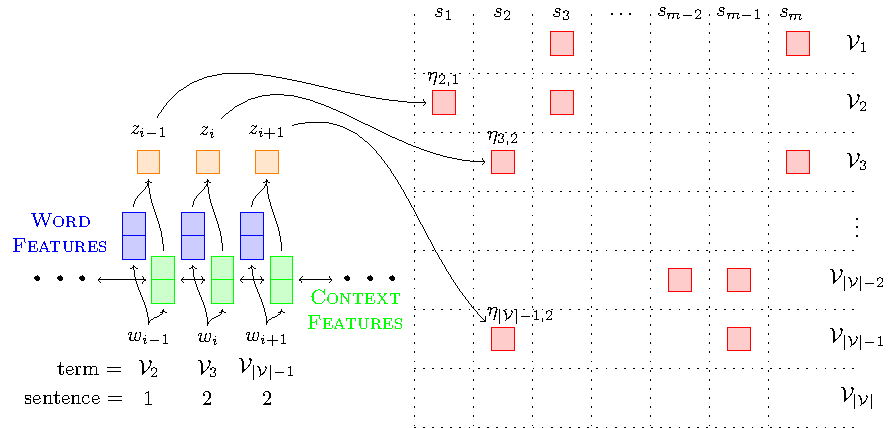
\includegraphics[scale=.7]{chapter4/figures/4_2_wimp_model.pdf}
 \end{center}
\caption{Left: Word and context features are extracted from the flat token
sequence representation to get word level importance scores 
$\wordImportance_i$. Right: word level scores are aggregated into a sparse
bag-of-words representation of the input sentences.}
\end{figure}

Our previous experiments revealed that lexical sematics were not the 
main driver of learning in sentence extractive news summarization. 
One could plausibly argue that it is a feature, not a bug, and that 
the structural
signals in news are intentional and not to be avoided. However, we think more 
attention could be paid to estimating importance scores at the word level.
We are motivated by potential application to abstractive generation: better
word level importance estimation could help to remove all but the most 
necessary content from the documents as a preprocessing stage before
abstractive summarization. We are also encouraged by parallel practices
in multi-lingual news summarization, where word importance weights 
are the main ingredient in sentence representations. 


\newcommand{\mlingsys}{\textsc{Classy}}

%\subsubsection{A brief discussion of \mlingsys.}

\mlingsys and its antecedents have been consistent top performers in various
summarization workshops \cite{tac,multiling}. In general the main approach 
is to represent each sentence as a sparse bag-of-words, where non-zero
entries correspond to word importance weights for the words found in the 
sentence. Typically, tf-idf weights are used for the importance scores.
The term by sentence matrix representing the document or documents to be
summarized is then factorized into two low rank matrices (typically with
non-negative entries) representing term factors and sentence factors.
The entries in the sentence factor matrix represent latent factors, 
and apriori the importance of each sentence is the sum of its latent factors.

Sentence selection can subsequently be performed using one of several methods.
In the naive case, one can select the sentence with the highest vector norm, 
substract the selected latent factors from the remaining sentence vectors
(zeroing out any terms that become negative), and repeating until the
summary length budget is reached. More sophisticated selection procedures
involving multi-dimensional knapsack packing or submodular optimization 
can be used, however these are not the focus of this work.

One draw back to this approach is that the sentence factors and word 
importance scores are unsupervised with respect to the final summarization
objective; their utility to the summarization task is a happy coincidence.
Additionally, the word importance scores are not assigned based on the 
context in which the word appears.

We propose to address these issues by learning word level importance 
scores in the process of single document sentence extractive summarization.
Additionally, we propose a method of adapting these scores from the 
single document case to multi-document summarization.

\subsubsection{Proposed Model}


In our proposed model for word importance, we estimate the importance of
each word in the context it occurs by first running the ELMO model
over all the words in the document to obtain contextual representations
of each word. The ELMO embeddings are then combined with pretrained Glove
embeddings, document frequency embeddings, topic signature embeddings,
sentence position embeddings, and part-of-speech tag embeddings and then
fed into a multi-layer perceptron to predict a scalar importance score.
When a word occurs multiple times in the input, it can be given a different 
importance score at each location because the ELMO embeddings will capture
contributions of the salient neighbor words. A term-sentence matrix is 
then formed from the input, using the estimated word importance scores 
as the term weights. A sentence extractive summary can be obtained 
using the naive sentence selection method described above or in Figure ?.
The total score for the summary can also be obtained.

We can train this summarizer using a gold extract sequence and a margin loss
\[  \max\left(0, 1 + f(\hat{y}) - f(y) \right) \] where $f(\hat{y})$ is
the score of our predicted extract summary.


Let $z_1, z_2, \dots, z_n$ be the bag of words representations of the 
sentences selected for the summary, in the order they were selected.
The score for the summary is computed as 
$\textsc{Score}(z) = \sum_{i=1}^n \sum_{j=1}^k \max(0, z_{i,j} - \sum_{l=1}^{i-1} z_{l,j})$ 


~\\
~\\

Let $\vocab$ be a fixed vocabulary of words. A document is a sequence $m$
words $\word = \{\word_1, \word_2, \ldots, \word_m\} \in \vocab^m$.
We define two mappings of words to dense vector representations.
The first $\fdef{\wordFeatures}{\vocab}{\Rn{d_1}}$ maps words to 
a concatenation of feature embeddings whose total dimension is of size $f$. 
The various components of the feature embeddings include the word's Glove 
embedding, an embedding for sentence position, and other features of the word.
The second mapping
$\fdef{\contextFeatures}{\vocab}{\Rn{d_2}}$ maps the word to it's contextual
embedding; here this corresponds to the output of \elmo at that word's
position in the document. 
The importance score $\wordImportance_i$ of a word $\word_i$ is the output of 
a feedforward layer 
\[ \wordImportance_i = \sigma\Big(W \left[\begin{array}{c} \wordFeatures(\word_i) \\ \contextFeatures(\word_i) \end{array} \right] + b \Big) \]
    where $W \in \Rn{d_1 + d_2}$ and $b \in \R$ are learned weight
and bias parameters, and $\sigma$ is the logistic sigmoid.

Next, we aggregate the flat token level scores into a bag-of-words (BOW) 
representation for each sentence in the document.
Let $I_i$ be the set of indices of the flat word sequence corresponding
to the words in $i$-th input sentence. Let $\bow_i$ be the BOW 
representation of the $i$-th sentence with entries 
\[ \bow_{i,j} = \begin{cases} 
    0 & \textrm{if $\word_k \ne \vocab_j $ for all $k \in I_i $} \\ 
\sum_{k \in I_i} \mathbbm{1}\{\word_k = \vocab_j \} \cdot \wordImportance_k  & \textrm{otherwise}     \end{cases} \]
        for all $j \in \{1, \ldots, |\vocab|\}$.



\begin{figure}
  \begin{algorithmic}[1]
    \Procedure{\textsc{BowExtracter}}{$\bow, \beta, \kappa$}
   
      \State $\bow_i^{(1)}  \gets \bow_i \quad \forall i \in [[n]]$
      \State $\hat{\eta} \gets 0$
      \State $t \gets 0$
      \While{ $\sum_{i=1}^t \kappa_{\predLabels_i} < \beta$ and $t < n$}
        \State $t \gets t + 1$
        \State $\predLabels_t \gets \operatorname{arg max}_{i \in [[n]]}
            \sum_{j=1}^{|\vocab|} \bow^{(t)}_{i,j}$
        \State $\bow_i^{(t+1)} \gets \max(0, \bow_i^{(t)} - \bow^{(t)}_{\predLabels_t} )\quad  \forall i \in [[n]]$
        \State $\hat{\eta} \gets \hat{\eta} + \sum_{j=1}^{|\vocab|} \bow_{\predLabels_t,j}^{(t)}$
         

      \EndWhile
        \State \Return $[\predLabels_1,\ldots,\predLabels_t], \hat{\eta}$ \Comment{Returns summary sentence indices and summary score.}
    \EndProcedure
  \end{algorithmic}
\caption{Simple sentence extraction algorithm given non-negative BOW inputs.}
\label{alg:wimp_ext_alg}
\end{figure}



        With the BOW representations in hand, we perform sentence selection
        using the algorithm presented in \autoref{alg:wimp_ext_alg} to 
        obtain a predicted extract indices $\predLabels$ and their associated
        score $\hat{\eta}$.

        We can optimize this model using a margin loss, where given a 
        gold extract sequence  $\labels$, we can compute the associated
        gold extract summary score $\eta$ and then minimize the following
        loss function \[\mathcal{L}_{ext}(\predLabels, \labels;\theta) = \max\big(0, 1 + \hat{\eta} - \eta\big)\]
        with respect to the parameters of the word importance predictor.
        If needed, we can also introduce a supervised learning signal to the 
        individual word importance scores by collecting labels $\zeta_i$ for
        each $\wordImportance_i$ such that $\zeta_i = 1$ if $\word_i$ occurs
        and any human reference abstract and $0$ otherwise. For the word level
        loss we would use the cross entropy 
        \[ \mathcal{L}_{word}(\wordImportance, \zeta; \theta) = -\sum_{i=1}^m \zeta_i \log \wordImportance_i + (1 - \zeta_i) \log (1 - \wordImportance_i). \] 




        \paragraph{Adaptation to MDS} We also propose a simple 
        self attention-based modification to
        the word importance aggregation step to help adapt this method
        to multi-document summarization (MDS). \citep{conroy} found
        that dimensionality reduction on the BOW representations improves
        summarizer performance in the MDS setting (but not on single document
        summarization). 


        We plan to experiment with the following importance 
        aggregation method. First, given the outputs of the contextual features
        $h_i$, we compute a self attention matrix $\Lambda \in \Rn{m\times m}$
        where \[\Lambda_{i,j} = \sigma(h_i \cdot h_j / \tau + b)  \]
        using sigmoidal attention \cite{strucattn} with a learned bias 
        parameter $b$ and a temperature parameter $\tau$.
        Next we compute an attention weighted word importance score $\bar{\wordImportance}_i$ for each word in the input using the following formula,
        \[ \bar{\wordImportance}_i = \sum_{j=1}^m \wordImportance_j \cdot \Lambda_{i,j}.\]

        Our motivation is that by accumulating scores based on context
        similarity, words and topics that appear in multiple documents 
        will accumulate the bulk of the word importance scores, giving 
        an added boost to sentences that contain them. Implicitly, errant
        words from one document that are not on topic to the cluster will
        effectively not contribute much to a sentences score, reducing the 
        effectve dimension of the BOW vectors and regularizing individual
        sentences to the document cluster's mean.

        
        Since we are training our models on single documents, we expect that
        running our pretrainined word scoring model on the individual 
        documents from an MDS document cluster will result in 
        minimal task-adaptation mismatch. Remaining bias and temperature
        parameters can easily be tuned on the small amount of MDS training 
        data available.

        We also plan to compare this method to using a non-negative matrix 
        factorization 
        method on the output of the learned BOW representation, 
        and to hard attention assignments using Brown clustering.







%\subsubsection{
%\cite{conroy} 


 

}{}

\section{Faithful Text Generation}
\label{sec:faithful_generation}

Sections~\ref{sec:feature_salience}~and~\ref{sec:deep_learning_salience}
have focused on identifying the most important content for summary inclusion,
while punting somewhat on summary generation -- and for good reason, 
extractive summarization minimizes the burden of creating fluent text. 
While abstractive text generation certainly adds significant challenges to 
summary creation, 
its benefits are many: the ability to achieve tighter compression ratios
for space constrained scenarios \citep{fan2017controllable}, the potential
to target different reading levels \citep{margarido2008automatic}
or style \citep{shen2017style}, and more pragmatically, in
an increasingly copy-protected web, abstractive generation may be the only 
legally viable option for content aggregation services 
\citep{kassam2014google}.

With this expressive power comes the danger that the generated text may
misconstrue the source material. Trust in machine learning
models is increasingly being recognized as an important factor in user 
adoption \citep{ribeiro2016should}, and mistakes of this kind will be 
a show stopper for downstream consumers of summarization (e.g. if an
abstractive summarization model in the previous crisis-monitoring scenario
erroneously attributes the location of a deadly earthquake). 

\begin{figure}
 \centering
 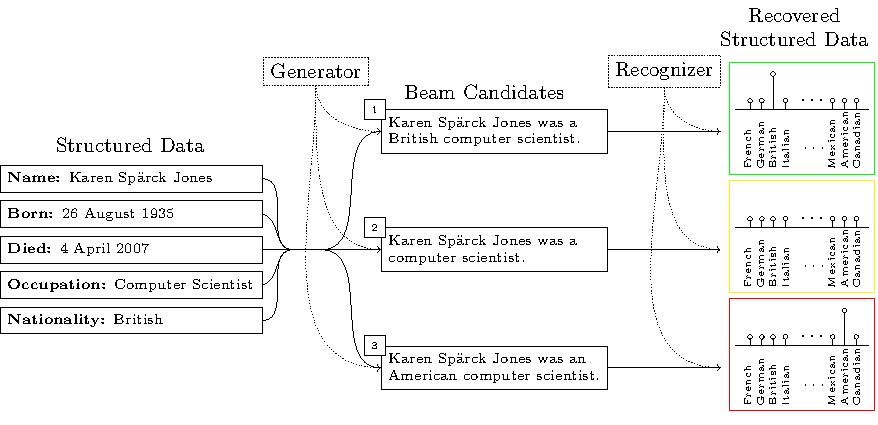
\includegraphics{images/faithful_generation/example1.pdf}
 \caption{Example of faithful generation from structured data. The generator
 is responsible for producing a list (beam) of candidate utterances from the 
 structured data. The recognizer reranks the beam candidates based on the 
 plausibility of the recovered structured data. }
 \label{fig:fgen_example1}
\end{figure}


As a potential solution,
we propose modeling text generation as a two player game between a generator
model and a recognizer model. %, akin to an auto-encoder \citep{rumelhart1985learning}. 
First, we provide as input to the 
generator some evidence (e.g., raw text or table data). 
Conditioned on the evidence, the generator must produce 
a list of candidate utterances accurately describing that evidence. The recognizer
scores the candidates based on its ability to reconstruct various 
pieces of the evidence. The generator receives supervision in the form of a 
reference utterance (i.e. standard sequence maximum likelihood training) 
and also from the recognizer scores across all candidate
utterances.
I.e., the generator learns to produce a variety of utterances that are
simultaneously fluent but also lead the recognizer to recover the original
evidence correctly. If we have an accurate recognizer, the generator should
improve in its ability to render truthful descriptions of the evidence.



% no alignments needed
% decompose supervision into fluency and truthfulness
% learn mutliple realizations that are fluent and correct.
% can experiment in controllable generation 
% can experiment with different soft constraints


There are several motivations for this approach. 
First, RNNs typically used to implement text generators are impressive
conditional language models and will generally learn to create fluent outputs.
By adding a faithfulness component (recognizer derived 
losses) to the learning objective we can hopefully improve reliability 
of text generation for downstream users. 

Second, by learning across
multiple (beam search) candidates, we can encourage the model to 
explore syntactically and lexically diverse paraphrases that are still
factually licensed by the evidence. We think this will be usefull when
text generation is part of a pipeline that may want to consider various 
realizations to ensure fluency and coherency at a macro, e.g. document, level.

Furthermore, the recognizer is itself a learned model; 
as text classification models improve, so will the faithful generation 
framework.
It does not require
alignments between the evidence and the reference utterances; it uses
the same evidence/utterance parallel data as the generator to train.
The recognizer can also be used to derive confidence scores 
for individual utterances if this is needed
in a downstream application. 


Finally, we think this framework also allows for an alternative approach
to controllable text generation. Currently, most controllable approaches
to generation rely on appending feature embeddings to the decoder 
input (e.g. for length \citep{fan2017controllable} or for syntactic 
structure \citep{colin2018generating}). By specifying a desired output from
the recognizer, we can train biased generators that adhere to soft constraints,
similar to these other methods.
What's more, the recognizer allows us to certify that individual outputs 
actually adhere to the desired constraints, something the input only control
mechanisms do not do.



%First we do not need 
%alignments between the evidence and the utterances, the recognizer can learn
%from 



%~\\
%~\\

%While we will experiment with a variety of loss functions to find something
%that works well empirically, we expect in principal to train the generator
%to maximize the expected likelihood of evidence under the recognizer.



See \autoref{fig:fgen_example1} for an example 
where we have table data as evidence (biographical data about name, nationality, and 
occupation), and we generate several plausible and implausible 
candidates that are evaluated by the recognizer.
The first candidate is 
 ranked highly because the recognizer can correctly infer that the 
 nationality of Karen Sp\"arck Jones is British (green box). The second 
 candidate is possibly fine because it maximizes entropy over the choice 
 of nationalies (yellow box), i.e. it makes no commitments either way and does
 not produce a non-true statement. The third beam candidate is clearly wrong
 as the recognizer infers that the nationality is American which is a false
 statement according to the true table data (red box).
 In some applications it may be OK to omit information, in which case the first
 and second utterances are acceptable and we only want to train the generator to
 avoid the third. In other cases, we may want to require that all input
 evidence has some corresponding description in the output, in which case,
 only the first utterance is acceptable. 
 The faithful generation framework allows us to learn what the correct possible outputs are  
 by specifying which recognizer distributions are acceptable. 

In the remainder of this section, we cover the related work in this area
before describing in more detail the faithful generation framework for 
data-to-text and text-to-text scenarios and our proposed experiments.
%formally define two faithful generation
%models, one for generating text from structured data and 
%one for generating text from  text data. We conclude by briefly describing some
%applications and datasets we will use to evaluate these modls.

\subsection{Related Work}

%In our proposed faithful generation framework, we use one model, the 
%generator, to
%create a text utterance, e.g. a summary of a document or a description
%of a data table, and another model, the recognizer, to answer questions 
%about the underlying document or table, using the utterance as evidence.
%A good utterance, then, is one that allows the recognizer on average to
%correctly answer those questions.

The conceptual underpinnings of faithful generation trace back to two
ideas in the NLP literature. The first is round-tripping in machine translation
\citep{somers2005round,rapp2009back}, i.e. a good translation system should be able to translate
a source language text to a target language text and then back to the source
language with minimal corruption between the original source and the 
back-translated source. \cite{andreas2016reasoning} have recently carried 
this idea 
over to explaining structured prediction tasks, where, e.g., 
the structure is a 
formal plan for a robotic agent; a rational speaker  generates the text
description of the plan that is most likely to lead a rational listener 
to correctly re-interpret the original plan. Faithful generation is similar:
the generator (speaker) 
 encodes an 
input object
(either text or data table) into 
an intermediate text representation, and the recognizer (listener) then tries to 
answer questions about the source using only the intermediate text.
The main difference is that in faithful generation, we are interested not in
a full reconstruction of the source from the intermediate representation, but
rather, the utility of the intermediate representation on a downstream task, 
e.g. question answering.


The other conceptual precedent is that of discriminative reranking 
of $n$-best lists \citep{collins2005discriminative,charniak2005coarse};
a generative model produces the $n$ most likely latent structures, e.g. parses,
and a discriminative model, which does not have the burden of modeling
the observations, rescores this list.  This idea has been applied 
to text generation as well. \cite{wen2015stochastic} and 
\cite{novikova2017e2e} use a 
sequence-to-sequence
model with beam search to generate $n$-best texts from either a 
dialogue plan or data table respectively,
 and then use a separately trained
classifier to downrank the beam candidates that do not correspond to the 
underlying
structured object.
%statements (according to the data table).
We argue that this is insufficient since we might want to consider 
all beam candidates in a downstream task, e.g. a macro content planner stage.
%that maximizes the  coherency of a sequence generated utterances.
For this model to provide linguistically interesting realizations that are 
still
factually true requires expanding the beam size 
which increases the computational and memory demands at test time. 
In our faithful generation framework, we directly discourage the generator from
ever allowing an untrue statement to be kept in the beam. This is done
using the recognizer directly as a learning signal and backpropagating
through the beam search process \citep{wiseman2016sequence}.

Increasingly, summarization researchers are exploring
 \textsc{Reinforce}-style
policy gradient methods to optimize non-differentiable metrics like 
\textsc{Rouge} \citep{paulus2017deep,arumae2018reinforced,kryscinski2018improving,narayan2018ranking,pasunuru2018multi}.
The most related to our work is that of \cite{arumae2018reinforced} 
and \cite{pasunuru2018multi}.
\cite{arumae2018reinforced} 
learn an extractive summarization model that maximizes
performance of a question-answering model on cloze style questions created
from the reference summaries. In our proposed method, the questions are 
generated from the source document and we use abstractively generated 
summaries as
the input to the question answering model, a significantly harder task.
\cite{pasunuru2018multi} learn an abstractive summarization model that
optimizes the likelihood that the generated summary is entailed by the 
ground-truth reference summary. The entailment likelihood is obtained from a
model trained on the SNLI \citep{bowman2015large} and MULTI-NLI 
\citep{williams2018broad} datasets.
This entailment measure is somewhat orthogonal to the faithful generation 
objective, as our proposed
approach directly evaluates the utility of the summary as a faithful proxy
for the underlying document, not the reference, which is the ultimate goal of the 
summarization task.


Most reinforcement learning applied to abstractive summarization uses
one Monte-Carlo sample from their policy distribution to estimate the 
expected reward. We propose to optimize
the entire beam search so that all beam candidates are viable in downstream
tasks. In this way, faithful generation also resembles 
minimum error rate training (MERT) \citep{och2003minimum} 
and minimum Bayes-risk decoding (MBD)
\citep{kumar2004minimum} in that we are reshaping a distribution of $n$-best
beam candidates to optimize the expected value of an evaluation metric.
We also plan on using reward shaping supervision from the recognizer
model to localize reward signals \citep{mnih2014neural} to specific spans of 
a candidate utterance
that are most responsible for violating the input document. Localized
reward shaping will help to penalize only the factually incorrect spans
and preserve syntactic and structural choices that are independent of 
such entailment considerations.


Other notable approaches to improving the faithfulness of abstractive 
generation include \cite{guo2018soft} who use a multi-task training objective 
to learn a shared decoder that can alternatively summarize a document,
generate a question about a document, or generate a logically entailed text 
from a document.
The latter task is relevant here, as the authors claim that this entailment
generation objective encourages the decoder to produce only logically entailed
summaries. This claim deserves further scrutiny as their human 
evaluation only asked about \textit{relevance} and \textit{fluency} where
the relevance criteria included topical relevance and redundancy in addition
to factual accuracy, confounding any interpretation of the generated summaries
as being more faithful to the source document.

%~\\
%This is done by learning from 
%Our proposed method is to learn from the recognizer's signals
%during training, i.e. backpropagating throught the beam search process
%so that the beam does not need to to be pruned during test time, i.e. 
%all surviving beam 
%candidates should be factually true.



%Similarly, minimum error rate training (MERT) \citep{och2003minimum} 
%and minimum Bayes-risk decoding 
%\citep{kumar2004minimum}
%rerank $n$-best translations in order to directly optimize an evaluation
%metric like \textsc{Bleu} \citep{papineni2002bleu}.

%Faithiful generation can be recast in the MERT framework by considering
%the evaluation metric to be the recognizer's classification accuracy on
%table data or cloze accuracy on text data. This is perhaps most similar
%to    



  \subsection{Structured Data Model}
  \label{sec:struct_data_model}

  Our structured data model consists of evidence/utterance tuples $(\evidence, \utterance)\in
  \dataset$.
   The evidence $\evidence = \{\evidence_1, \ldots, \evidence_m\}$
   is a sequence of $m$ categorical variables drawn from  
   $\evidenceSpaces{m}$ where $\evidence_i$ is the observed value for the 
   $i$-th field in the structured data, e.g. the $i$-th field could correspond 
   to \textit{occupation} with possible values
   in $\evidenceSpace_i = 
   \{ \textsc{Accountant}, \textsc{Actor},
    \ldots, \textsc{Zoologist} \}$ .
The utterance $\utterance = \{\utterance_1,\ldots, 
\utterance_{|\utterance|}\}$ is a 
  sequence of $|\utterance|$ tokens with each token drawn from a fixed 
  vocabulary $\vocab$. The utterances correspond to natural language 
  realizations of a subset
  of the evidence.

  The first player in our game is the \textit{generator} $\gen$, which can 
  generate a list of $k$ candidate utterances $\utterance^{(1)},\ldots,
  \utterance^{(k)}$. In practice, $\gen$ is a sequence-to-sequence 
  model \citep{bahdanau2014neural} with parameters $\genParams$, and the $k$ 
candidates are produced using beam search.
 The second player, called the \textit{recognizer}, has a mapping
 $\fdef{\rec_i}{\vocab^*}{(0,1)^{|\evidenceSpace_i|}}$ of utterances to
 probabilities over values for each field
 $i \in \Idx{m}$. We say that an utterance $\utterance$ is \textbf{faithful}
 to the evidence $\evidence$ under a recognizer $\rec$, 
denoted $\faithful(\utterance,\evidence,\rec)$, if, for all $i\in \Idx{m},$
\[ \rec_i(\evidence_i|\utterance) >
 \max_{\evidence^\prime \in \evidenceSpace_i \setminus \{\evidence_i\}}
  \rec_i(\evidence^\prime|\utterance) 
  \quad \textrm{ or } \quad  
  \entropy^{(i)}_{\max} - \entropy_{\rec_i(\cdot|\utterance)} < \epsilon\]
where $\entropy^{(i)}_{\max}$ is the maximum entropy for the $i$-th field,
i.e. the entropy of the uniform distribution 
$\log |\evidenceSpace_i|$, and $\entropy_{\rec_i(\cdot|\utterance)}$ 
is the entropy of $\rec$ over the $i$-th field. In English, 
an utterance is faithul to the evidence if the recognizer can correctly
predict the true evidence from the utterance (left statement) or, barring that,
the recognizer can not infer a value of the evidence with
anything better than random chance (right statement).

We evaluate the degree to which the generator is faithul with the quantity
\[ \objective_\beamDistr(\evidence) = \E_{\utterance \sim \beamDistr(\evidence)} 
 \Ind{\faithful(\utterance, \evidence, \rec)}, \]
where $\beamDistr(\evidence) \propto \frac{\gen(\utterance|\evidence;\genParams)}{|\utterance|}$ is a the generator distribution renormalized by average token
probability over the
beam candidates $\utterance^{(1)},\ldots, \utterance^{(k)}$.

We implement the recognizer using CNN classifiers with parameters $\recParams$,
 and fit the parameters  with 
the average log likehood objective \[ \objective_\rec(\phi) = 
\frac{1}{|\dataset|} \frac{1}{m} \sum_{\evidence, \utterance \in \dataset} \sum_{i=1}^m 
\log \rec_i(\evidence_i|\utterance;\recParams).\] After training, the 
recognizer is frozen and we do not update the parameters when fitting the 
generator.

The generator is pre-trained also using the standard maximum log likelihood
objective: \[\objective_\gen(\genParams) = 
\frac{1}{|\dataset|} \sum_{\evidence, \utterance \in \dataset} 
\log \gen(\utterance|\evidence;\genParams).\] To make the generator faithful,
we then maximize the joint objective \[
\frac{1}{|\dataset|} \sum_{\evidence, \utterance \in \dataset} 
\Big[
\log \gen(\utterance|\evidence;\genParams) + 
 \E_{\utterance \sim \beamDistr(\evidence)} 
 \Ind{\faithful(\utterance, \evidence, \rec)} \Big], 
\]
where the second term results in a minimum risk training (MRT) style gradient
update \citep{edunov2018classical}.






\subsection{Text-to-Text Model}
For cases where the evidence is not structured data but text, e.g. 
summarization, we can modify the data-to-text model slightly to obtain 
a workable faithful training regime. Our data will now consist of 
4-tuples $(\evidence, \utterance, \bar{\evidence}, \bar{\utterance}) \in 
\dataset$ where $\evidence$ is the input text to be summarized, 
$\utterance$ is the reference
abstractive summary, and $\bar{\evidence}, \bar{\utterance}$ are cloze
style questions and answers \citep{taylor1953cloze} respectively. In
a typical cloze question, a passage is given followed by a sentence with a 
missing word; one must provide the correct word to fill in the blank 
based
on evidence from the passage. We can heuristically create cloze style questions
for summarization by selecting input phrases/sentences with high similarity
to the reference summary, and redacting random content words. See 
\autoref{fig:cloze_example} for an example from the CNN/DailyMail dataset.



We modify our recognizer definition to the following:
an utterance $\utterance$ is \textbf{faithful}
 to the evidence $\evidence$ under a recognizer $\rec$, 
denoted $\faithful(\utterance,\evidence,\rec)$, if
\[ \rec(\bar{\utterance} |\bar{\evidence}, \utterance) >
 \max_{\bar{\utterance}^\prime \in \vocab \setminus \{\bar{\utterance}\}}
\rec(\bar{\utterance}^\prime |\bar{\evidence}, \utterance)
  \quad \textrm{ or } \quad  
  \entropy_{\max} - \entropy_{\rec(\cdot|\bar{\evidence}, \utterance)} < \epsilon\]
where the entropy terms are defined similarly to 
\autoref{sec:struct_data_model} and the recognizer is now modified to map 
cloze question/passage tuples $\bar{\evidence},\utterance$ to probabilities
of a cloze answer
$\bar{\utterance}$. In practice multiple cloze question/answer pairs will
be created for each input/summary pair. Training of the faithful generator
will proceed similarly to the process outlined in \autoref{sec:struct_data_model}.

We plan to perform faithful summary generation
first using the TL;DR dataset \citep{volske2017tl} which contains over 2 
million
Reddit comments with summarizations. Since the comments being summarized
are shorted than most news articles, we think this will be a more tractable
starting point for validating the utility of the cloze task.
Following this, we would like to apply this technique to
the CNN/DailyMail, NYT, and Newsroom datasets 
\citep{hermann2015teaching,sandhaus2008new,grusky2018newsroom} since
these datasets are large enough to train abstractive summarizers.
As in the data-to-text experiments, we will also include a human evaluation
of the beam candidates to ensure that the training does indeed produce
a distribution of faithful outputs.

%
 \subsection{Applications and Data}
We envision several applications and scenarios where faithful generation might
be useful. The first is for data-to-text generation tasks. We plan on 
training the structured data model on at least two data-to-text tasks. 
The first is a biography generation task using biographical Wikipedia
entries and structured data extracted from the corresponding Wikipedia page's
info box \citep{lebret2016neural}. The second data-to-text task is a 
restaurant description generation task, where the structured data consists
of data about restaurants (types of food offered, location, etc.) 
\citep{novikova2017e2e}.
For the text-to-text scenarios, we plan to perform faithful summary generation
first using the TL;DR dataset \citep{volske2017tl} which contains over 2 
million
Reddit comments with summarizations. Since the comments being summarized
are shorted than most news articles, we think this will be a more tractable
starting point for validating the utility of the cloze task.
Following this, we would like to apply this technique to
the CNN/DailyMail, NYT, and Newsroom datasets 
\citep{hermann2015teaching,sandhaus2008new,grusky2018newsroom}.


We would also like to explore ways in which faithful generation could 
be applied to understanding and controlling for bias in machine learning
\citep{bolukbasi2016man}. By modifying the faithful generation objective
function to reward only uncertainty for missing data fields, we could 
encourage the generator to produce utterances that are decorrelated with 
a particular field value. 
As an example let's say that our observed evidence consists
of $\evidence_{name} = \textsc{Fran Allen}$ and  
$\evidence_{occupation} = \textsc{Computer Scientist}$
but we did not know the value of the gender field, 
$\evidence_{gender} = \textsc{Missing} $. If our dataset over 
represents men (a known bias in Wikipedia), 
the sequence-to-sequence based generator is 
likely to fall back to the most prevalent patterns in the dataset and use
the masculine pronoun during generation. In turn, 
the gender field recognizer is likely
to key in on pronoun usage as a discriminative feature and predict male.
If we train the faithful generator to produce utterances that result in
maximum uncertainty in the gender 
recognizer then it is likely to avoid gendered pronouns and minimize
the chances of implying incorrect knowledge.



\pagebreak
\section{Research Plan}
Research plan.

\section{Conclusion}

In this thesis we have proposed to tackle two central problems for 
summarization: selecting salient information for summary inclusion and
generating text that is grounded in the underlying structured or text data. 
Our experiments on the salience problem spans many different summarization
scenarios, including the very challenging stream summarization task.
We also show how to incorporate salience estimation into two very different
paradigms, exemplar based clustering and learning-to-search.
We also contribute analysis as to the behavior of several deep learning models
of sentence salience, and,  based on these experiments, propose a novel
word importance estimation model, with applications to single and 
multi-document summarization. We hope that these sections of the thesis
form a flexible collection of strategies useful to a broad range of 
researchers in summarization. This work is diminished, however,
if we do not
have robust generation algorithms that do not hallucinate information.
We believe the final chapter on faithful generation will prove a useful 
paradigm for dealing with errorful generation outputs. We also believe
that faithful generation can be useful on a variety of text generation tasks
beyond just summarization, e.g. data-to-text generation.



\bibliographystyle{plainnat}
\bibliography{cites}

\end{document}
